%%-----------------------------------------------------------------------
% Loading the packages and classes
%%-----------------------------------------------------------------------

\documentclass[12pt,oneside,a4paper,final]{book}%
%\usepackage{glossaries}
\usepackage{a4}%                        %% Verwendet mehr Platz auf einer A4 Seite als Option a4paper in book
%\usepackage[english,ngerman]{babel}%    %% Babel Sprachen
\usepackage[T1]{fontenc}
\usepackage{amssymb}%                   %% AMS Symbole
\usepackage{amsmath}%                   %% AMS Math Funktionen
\usepackage{amsfonts}%
\usepackage[Sonny]{fncychap}%           %% Chapter Style
\usepackage[english,noprefix]{nomencl}%  %% Nomenclature (Symbolverzeichnis)
\usepackage{makeidx}%                   %% Index
\usepackage{graphicx}%                  %% Graphiken
\graphicspath{{img/}}
\DeclareGraphicsExtensions{.pdf,.jpeg,.png,.jpg}
\usepackage{psfrag}%                    %% Tex-Schriftarten und Formeln in EPS-Grafiken
\usepackage{color}
\usepackage{nicefrac}
\usepackage{ifthen}
\usepackage{fancyhdr}\usepackage{amsmath}
\usepackage{amsfonts}
\usepackage{amssymb}
\usepackage{subfigure}
\usepackage[xindy, acronym, toc]{glossaries}
\usepackage{cite}
\usepackage{listings}
\usepackage{color}
\usepackage[dvipsnames]{xcolor}
\usepackage{rotating}
\usepackage[ansinew]{inputenc}
\usepackage{tocbibind}
\usepackage{amsmath}
\usepackage{float}
\usepackage{titlesec}
\usepackage{booktabs}
\usepackage{pdfpages}
%%Define Acronyms like
\newacronym{tgm}{TGM}{Technologisches Gewerbemuseum}
% use on every place in your document \gls{mas} for TGM or - for plural - use \glspl for TGMs
% at the first usage of this, the acronym will be introduced, everywhere else it will only be the in the short form: ``Technologisches Gewerbemuseum (TGM)''
% TIPP: USE THIS FOR EVERY NAME/SOFTWARE-TOOL/MAIN PART OF YOUR WORK, like JAVA, - so that, e.g. JAVA is not written Java everywhere else in your thesis.
\newacronym{gis}{GIS}{Gotti is supa!}
%%-----------------------------------------------------------------------
% Using the Hyperref-Package for PDF-Online Version
%%-----------------------------------------------------------------------
\def\usehyperref{1}

\ifnum\usehyperref=1
\usepackage[pdftex=true,
  pdftitle={Diplomarbeitas},
  pdfauthor={Thomas Pokorny},
  bookmarksopen,
  colorlinks,
  citecolor=blue,
  linkcolor=blue,
  breaklinks%
]{hyperref}%
\fi


% listings configuration
\lstset{
	basicstyle=\fontfamily{DejaVuSansMono}\fontshape{n}\fontseries{m},
	numbers=left,
	numberstyle=\small\color{gray},
	commentstyle=\color{gray},
	breakatwhitespace=false,         % sets if automatic breaks should only happen at whitespace
	breaklines=false,                 % sets automatic line breaking
	stringstyle=\color{red},     % string literal style
	rulecolor=\color{black},         % if not set, the frame-color may be changed on line-breaks within not-black text (e.g. comments (green here))
	keywordstyle=\color{blue}       % keyword style
}
%%-----------------------------------------------------------------------
% Rearranging Nomenclature
%%-----------------------------------------------------------------------


%\renewcommand{\nomname}{List of symbols}
%\renewcommand{\nompreamble}{The following list only contains symbols
%  that are used continuously throughout the text. Local symbols are
%  not listed.}
%\renewcommand{\nomgroup}[1]{
% \ifthenelse{\equal{#1}{A}}{\item[\textbf{General symbols}\bigskip]}{
% \ifthenelse{\equal{#1}{B}}{\item[\bigskip\bigskip\textbf{Chapter 2}\bigskip]}{
% \ifthenelse{\equal{#1}{C}}{\item[\bigskip\bigskip\textbf{Chapter 3}\bigskip]}{
% \ifthenelse{\equal{#1}{D}}{\item[\bigskip\bigskip\textbf{Chapter 4}\bigskip]}{
% \ifthenelse{\equal{#1}{E}}{\item[\bigskip\bigskip\textbf{Chapter 5}\bigskip]}{
% \ifthenelse{\equal{#1}{F}}{\item[\bigskip\bigskip\textbf{Appendix}\bigskip]}{
% }}}}}}}
%\makenomenclature



%%-----------------------------------------------------------------------
% Makes Bibliography available in Winedt
%%-----------------------------------------------------------------------

%GATHER{bib_kiefer.bib}


%%-----------------------------------------------------------------------
% Definition of possible environments
%%-----------------------------------------------------------------------

\newtheorem{theorem}{Theorem}[chapter]
\newtheorem{acknowledgement}{Acknowledgement}[chapter]
\newtheorem{algorithm}{Algorithm}[chapter]
\newtheorem{axiom}{Axiom}[chapter]
\newtheorem{case}{Case}[chapter]
\newtheorem{claim}{Claim}[chapter]
\newtheorem{conclusion}{Conclusion}[chapter]
\newtheorem{condition}{Condition}[chapter]
\newtheorem{conjecture}{Conjecture}[chapter]
\newtheorem{corollary}{Corollary}[chapter]
\newtheorem{criterion}{Criterion}[chapter]
\newtheorem{definition}{Definition}[chapter]
\newtheorem{example}{Example}[chapter]
\newtheorem{exercise}{Exercise}[chapter]
\newtheorem{lemma}{Lemma}[chapter]
\newtheorem{notation}{Notation}[chapter]
\newtheorem{problem}{Problem}[chapter]
\newtheorem{proposition}{Proposition}[chapter]
\newtheorem{remark}{Remark}[chapter]
\newtheorem{solution}{Solution}[chapter]
\newtheorem{summary}{Summary}[chapter]
\newenvironment{proof}[1][Proof]{\noindent\textbf{#1.} }{\ \rule{0.5em}{0.5em}}

\renewcommand{\chaptermark}[1]{\markboth{\thechapter.\ #1}{}}
\renewcommand{\sectionmark}[1]{\markright{\thesection.\ #1}}




%%-----------------------------------------------------------------------
% Marking of overfull boxes and increasing of tolerances
%%-----------------------------------------------------------------------

% F�r die Final-Version die n�chste Zeile auskommentieren um schawarze Balken (TU-Logo im Titelblatt) zu ignorieren!
\overfullrule=10pt%                     %% Markiert �berf�llte Boxen. z.b. hbox overfull (Evtl. nicht im pdf sichtbar!!!!)
\hfuzz=1pt%                             %% Toleranz bei hbox overfull erh�ht 1pt entspr. ca. 1/3 mm


%%-----------------------------------------------------------------------
% Counter
%%-----------------------------------------------------------------------

\titleformat{\chapter}[display]
  {\bfseries\huge}
  {\filleft\Large\chaptertitlename~\thechapter}
  {3ex}
  {\titlerule\vspace{1.5ex}\filleft}
  [\vspace{1ex}\titlerule]
  

\setcounter{secnumdepth}{3}%
\setcounter{tocdepth}{3}%



% Clear Header Style on the Last Empty Odd pages
\makeatletter
\def\cleardoublepage{\clearpage\if@twoside \ifodd\c@page\else%
    \hbox{}%
    \thispagestyle{empty}%              % Empty header styles
    \newpage%
    \if@twocolumn\hbox{}\newpage\fi\fi\fi}
\makeatother

%%-----------------------------------------------------------------------
% Avoid indents
%%-----------------------------------------------------------------------

\setlength{\parindent}{0pt}

%%-----------------------------------------------------------------------
%% Hyphenation for german abstract
%%-----------------------------------------------------------------------

\hyphenation{Fa-mi-lie
             Ski-bil-dung
             Ar-beits-wal-ze
             neg-lec-ted
             se-par-ate
             di-men-sio-nal
             her-r\"uhren
             N\"a-herungs-l\"os-ungen
             wissen-schaft-licher
             Regelungs-technik
             re-con-fi-gur-abili-ty
             manage-ment
             manu-facturing
             not-wendigen
             }


%%-----------------------------------------------------------------------
% Colored grafix
% 1 = color
% 0 = grey
%%-----------------------------------------------------------------------


\def\colorsw{1}

%%-----------------------------------------------------------------------
% Additional remarks
% 1 = with remarks
% 0 = without remarks
%%-----------------------------------------------------------------------


\def\addnotes{0}


%%-----------------------------------------------------------------------
% Define month
%%-----------------------------------------------------------------------

\def\monthdis{Mai 2014}

\makeglossaries
%%-----------------------------------------------------------------------
% Document
%%-----------------------------------------------------------------------


\begin{document}%
%\selectlanguage{english}%
\renewcommand{\indexname}{Index}%
\topmargin15.0mm
\oddsidemargin20.5mm
\def\tpdefault{{\sf \center \vspace*{-4cm}
%\begin{center}
%\hspace*{-1.3cm}
%\rule{17cm}{0.02cm}
%\end{center}


\begin{figure}[h]
\begin{flushright}	
		
\includegraphics[width=0.3\textwidth]{graphics/title/tgmlogo2.png}
	\label{fig:tgmlogo}
\end{flushright}
\end{figure}


\vspace{2cm}


{\Large %\bf 
DIPLOMARBEIT\\ \vspace{0.7cm}}
 {\LARGE \sloppy
{\bf \sf  \textbf{NAVAR}  %Wie hei�t unsere Diplomarbeit
\\}}
%
%
\vspace*{2cm}
{\normalsize Ausgef\"uhrt in Zuge der Reife und Diplompr\"ufung\\
Ausbildungszweig Systemtechnik\\ %unzutreffendes streichen
  \vspace{1.5cm}
  \normalsize unter der Leitung von\\
  \large Prof.\ Dr.\ Helmut Vana\\ 
  \normalsize Abteilung f�r
  Informationstechnologie\\
  \vspace{1.5cm}
  eingereicht am  Technologischen Gewerbemuseum Wien\\
  H\"ohere Technische Lehr- und Versuchsanstalt\\
  Wexstrasse 19-23, A-1200 Wien\\
  }}}


\begin{titlepage}
	\tpdefault
	{\sf \center \vspace{1.0cm}
	\normalsize von\\
	\large 
	Dominik George, 5AHITT\\
	Thomas Pokorny, 5AHITT\\
	Michael Fegerl, 5AHITT\\
	Aliaksei Korabach, 5AHITT\\
	\vspace {2 cm}
	\bf \sf {Wien, im Mai 2014} \\
		%	\vspace{2cm}
	%	\rule{\textwidth}{0.01cm}
	
	}
\end{titlepage}



\begin{titlepage}
	{\color{white}.}
	\bigskip
	\vspace{14cm}
	%\vfill%
	\noindent%

	Abteilungsvorst\"andin:\hfill Prof. Dr. G{\"u}nther ZANDRA \\
	\bigskip
	\bigskip

	Tag der Reifepr�fung:\hfill 11.06.2014-12.06.2014\\
	\bigskip
	\bigskip

	Pr�fungsvorsitzende:\hfill
    MinR Mag. Sabine NIEMEYER \\
	\smallskip

	Erster Gutachter:\hfill Prof. Dr. Helmut VANA\\
	\smallskip

	Zweiter Gutachter:\hfill Prof. Mag. Hans BRABENETZ\\
		\smallskip
\end{titlepage}

\frontmatter%   %% front matter will be numbered in small Roman letters

%%-----------------------------------------------------------------------


%%TCIDATA{OutputFilter=latex2.dll}
%TCIDATA{Version=5.00.0.2552}
%TCIDATA{LaTeXparent=0,0,Dissertation_SW.tex}


\chapter*{Vorwort}

Diese Arbeit wurde im Jahr 2012 im Zuge unserer Ausbildung in der Abteilung f�r Informationstechnologie am tgm, HTBLVA Wien 20, durchgef�hrt. 


\bigskip

Dankesworte

\bigskip
\bigskip
\bigskip
\bigskip



Wien, im \monthdis \hfill Name, Name, Name, Name \vfill
%

\thispagestyle{empty}
\vspace*{2cm}
\begin{center}
{\bf \sf \huge Erkl{\"a}rung}
\end{center}
{\sf \vspace{1cm} Hiermit erkl{\"a}ren wir, dass die vorliegende
Arbeit ohne unzul{\"a}ssige Hilfe Dritter und ohne Benutzung
anderer als der angegebenen Hilfsmittel angefertigt wurde. Die aus
anderen Quellen oder indirekt �bernommenen Daten und Konzepte sind
unter Angabe der Quelle gekennzeichnet.

Die Arbeit wurde bisher weder im In- noch im Ausland in gleicher
oder in {\"a}hnlicher Form in anderen Pr{\"u}fungsverfahren
vorgelegt.
\\[1.5cm]
Wien, im 2014
\\[2cm]
Michael Fegerl
\\[2cm]
Dominik George
\\[2cm]
Aliaksei Korabach
\\[2cm]
Thomas Pokorny
\\[2cm]
}%end sf

\chapter*{Abstract}

Augmented reality is a future oriented technology which allows to integrate digital information onto the view of the real-world. The potential uses for this technology are nearly endless, from video games, designers and retailers to health-care companies. Even if AR is a comparatively young technology their are already various different Applications which made use of it.          
\\

The purpose of the presented diploma thesis is to describe the usage of this technology in an Android mobile application. The project of developing the app was made in cooperation with our client 4relation Consulting GmbH. Our client recommended to use the Metaio SDK as AR-technology. Metaio is the worldwide leader in Augmented Reality research and technology with over 80 000 developers.
\\

The main function of the mobile application is to track cars (tracking is the process of recognizing objects with a camera). After the successful recognition the user is able to view diverse information of the auto-mobile. These information get loaded from a NAV database in which they are stored. The client is going to show the application together with the NAV database connection in his business presentations        %
%\selectlanguage{ngerman}%
\chapter*{Kurzfassung}

Die vorliegende Diplomarbeit befasst sich mit der Technologie Augmented Reality, die in einer Mobil Applikation verwendet wird. Momentan ist die Technologie Augmented Reality im IT Markt sehr stark Nachgefragt. In der Zukunft wird die Technologie auch in mobil Anwendungen implementiert. Die Arbeit wird in Kooperation mit einer wichtig gestellten Industrie namens 4relation Consulting GmbH durchgef{\"u}hrt. Die Modernen Smartphones,  sind die Ger{\"a}te  auf denen man Augmented Reality Anwendung nutzen kann. In Rahmen dieser Diplomarbeit wird beschrieben wie man Augmented Reailty mit der Metaio SDK f{\"u}r eine Mobile Anwendung verwenden kann. Des Weiteren bieten Mobileger{\"a}te  immer mehr Grafik -- und Rechenleistung und haben damit das Potential einer nahezu idealen AR-Plattform. Die Mobile Ger{\"a}te haben nur einen Bruchteil der Leistung eines Desktop -- PC's, aber dennoch gen{\"u}gend, um verschiedene Trackingverfahren durchzuf{\"u}hren. In dieser Arbeit wird beschrieben wie man ein Trackingsystem anwendet um ein Objekt zu erkennen. Ziel ist es von diesem Projekt ,dass man einen Fahrzeug durch das Trackingsystem erkennt. Die mobil Applikation soll ein Fahrzeugmodell erkennen und nachher die Information vom jeweiligem Auto am Display ausgeben. Um solch eine Applikation umzusetzen werden Wissen und Technologien aus verschiedensten Teilen der Informatik ben{\"o}tigt. F{\"u}r das Trackingsystem wird die Logik von der Metaio GmbH verwendet. Diese Firma bietet eine SDK an um solche Trackingverfahren in einer mobilen Anwendung einzubauen.%
%\selectlanguage{english}%


%%-----------------------------------------------------------------------
% Define Header for Content chapter
%%-----------------------------------------------------------------------


\makeatletter
\def\tableofcontents{\chapter*{\contentsname\@mkboth{\contentsname}{\contentsname}}
  \@starttoc{toc}}
\makeatother

\clearpage%
\setcounter{tocdepth}{1}
\tableofcontents
\clearpage
\listoffigures
\clearpage
\addcontentsline{toc}{chapter}{Listings}
\lstlistoflistings
\clearpage 
%\markboth{Contents}{Contents}


%\addcontentsline{toc}{chapter}{\numberline{}\listfigurename}%
%\listoffigures
%\listoftables%
%\addcontentsline{toc}{chapter}{\numberline{}\listtablename}%
%\clearpage%


%
\nomenclature[aa]{$t$}{time}
\nomenclature[bb]{$t_0$}{reference time}
\nomenclature[aa]{$m$}{mass}
\nomenclature[aa]{$\rho$}{mass density}

%%%%%%%%%%%%kommented KORA
%\markboth{\nomname}{\nomname}%
%\addcontentsline{toc}{chapter}{\numberline{}\nomname}%
%\printnomenclature


\mainmatter%   %% main part will be numbered in Arabic letter


% include chapters
% Chapter1
\chapter{Introduction} \label{chapter:introduction}

\begin{quotation}

``In the long history of humankind those who learned to collaborate and improvise most effectively have prevailed''

\begin{flushright}
(Charles Darwin)
\end{flushright}

\end{quotation}



Jetzt f�gen\footnote{asdsdakjadslhksfdjdf1}  wir etwas aus dem Intenet ein, das im Kapitel \ref{background} kommt\footnote{sdkjhkahfklsd2}: 

\begin{figure}[htbp]
	\centering
		
\includegraphics[width=0.40\textwidth]{graphics/title/tgmlogo.pdf}
	\caption[TGM Logo]{Da TGM Logo als Vektorgrafik, Schrift in schwarz, pfeil in blau und mehr mag ich nciht mehr schrieben.,.,.}
	\label{fig:tgmlogo}
\end{figure}

Wie schon klar war, 
bklala�dsafdsa�ladsf 
dsafmkdskjdsajhdsaf 
bal-. \cite{test}

Wir alle finden  \cite{koppensteiner_knowledge_2011, merdan_kasa_2009, bellifemine_book2_2007}.

Anmeldung zur Projektwoche am Turnersee \cite{bellifemine_book2_2007}
Als Erziehungsberechtigte(r) meines Sohnes (meiner Tochter)/ als Eigenberechtigte(r) gebe ich die Zustimmung, dass die Hin- und R�ckreise zum oder vom Kursort mit Autobussen erfolgt. Ebenso gebe ich die Zustimmung, dass diese(r) von einer eventuellen Ausgehm?glichkeit vom Heim in den Ortsbereich bei aufgehobener Aufsichtspflicht der begleitenden Lehrpersonen Gebrauch machen darf.
Ich nehme zur Kenntnis, dass f�r die gesamte Dauer einer Schulveranstaltung Alkoholverbot besteht. Das Rauchen in der Unterkunft ist nicht erlaubt \cite{koppensteiner_knowledge_2011}. Ich erkl?re mich einverstanden, dass mein Sohn (meine Tochter)/ich bei groben Verst??en gegen die Anordnung der Aufsichtspersonen und gegen die Heimordnung auf meine Kosten mit einer Begleitperson nach Hause geschickt oder von einem Erziehungsberechtigten/Elternteil vom Kursort abgeholt wird/werde. In dringenden F?llen bin ich mit der Heranziehung eines Arztes und notwendigen ?rztlichen Veranlassungen am Veranstaltungsort einverstanden. Bei Nicht-Teilnahme besteht die Pflicht zum Ersatzunterricht.
F�r alle sich dabei ergebenden Ereignisse und Folgen �bernehme ich als Erziehungsberechtigter die volle Verantwortung. Ein Betrag  von 160  liegt bei.

Anmeldung zur Projektwoche am Turnersee
Als Erziehungsberechtigte(r) meines Sohnes (meiner Tochter)/ als Eigenberechtigte(r) gebe ich die Zustimmung, dass die Hin- und R�ckreise zum oder vom Kursort mit Autobussen erfolgt. Ebenso gebe ich die Zustimmung, dass diese(r) von einer eventuellen Ausgehm?glichkeit vom Heim in den Ortsbereich bei aufgehobener Aufsichtspflicht der begleitenden Lehrpersonen Gebrauch machen darf.
Ich nehme zur Kenntnis, dass f�r die gesamte Dauer einer Schulveranstaltung Alkoholverbot besteht. Das Rauchen in der Unterkunft ist nicht erlaubt. Ich erkl?re mich einverstanden, dass mein Sohn (meine Tochter)/ich bei groben Verst??en gegen die Anordnung der Aufsichtspersonen und gegen die Heimordnung auf meine Kosten mit einer Begleitperson nach Hause geschickt oder von einem Erziehungsberechtigten/Elternteil vom Kursort abgeholt wird/werde. 

\begin{itemize}
	\item In dringenden F?llen bin ich mit der Heranziehung eines Arztes und notwendigen ?rztlichen Veranlassungen am Veranstaltungsort einverstanden. Bei Nicht-Teilnahme besteht die Pflicht zum Ersatzunterricht.
   \item F�r alle sich dabei ergebenden Ereignisse und Folgen �bernehme ich als Erziehungsberechtigter die volle Verantwortung. Ein Betrag  von 160 liegt bei.
\end{itemize}

\clearpage 
Anmeldung zur Projektwoche am Turnersee
Als Erziehungsberechtigte(r) meines Sohnes (meiner Tochter)/ als Eigenberechtigte(r) gebe ich die Zustimmung, dass die Hin- und R�ckreise zum oder vom Kursort mit Autobussen erfolgt. Ebenso gebe ich die Zustimmung, dass diese(r) von einer eventuellen Ausgehm?glichkeit vom Heim in den Ortsbereich bei aufgehobener Aufsichtspflicht der begleitenden Lehrpersonen Gebrauch machen darf.
Ich nehme zur Kenntnis, dass f�r die gesamte Dauer einer Schulveranstaltung Alkoholverbot besteht. Das Rauchen in der Unterkunft ist nicht erlaubt. Ich erkl?re mich einverstanden, dass mein Sohn (meine Tochter)/ich bei groben Verst??en gegen die Anordnung der Aufsichtspersonen und gegen die Heimordnung auf meine Kosten mit einer Begleitperson nach Hause geschickt oder von einem Erziehungsberechtigten/Elternteil vom Kursort abgeholt wird/werde. In dringenden F?llen bin ich mit der Heranziehung eines Arztes und notwendigen ?rztlichen Veranlassungen am Veranstaltungsort einverstanden. Bei Nicht-Teilnahme besteht die Pflicht zum Ersatzunterricht.
F�r alle sich dabei ergebenden Ereignisse und Folgen �bernehme ich als Erziehungsberechtigter die volle Verantwortung. Ein Betrag  von 160 liegt bei.\\

Anmeldung zur Projektwoche am Turnersee
Als Erziehungsberechtigte(r) meines Sohnes (meiner Tochter)/ als Eigenberechtigte(r) gebe ich die Zustimmung, dass die Hin- und R�ckreise zum oder vom Kursort mit Autobussen erfolgt. Ebenso gebe ich die Zustimmung, dass diese(r) von einer eventuellen Ausgehm?glichkeit vom Heim in den Ortsbereich bei aufgehobener Aufsichtspflicht der begleitenden Lehrpersonen Gebrauch machen darf.
Ich nehme zur Kenntnis, dass f�r die gesamte Dauer einer Schulveranstaltung Alkoholverbot besteht. Das Rauchen in der Unterkunft ist nicht erlaubt. Ich erkl?re mich einverstanden, dass mein Sohn (meine Tochter)/ich bei groben Verst??en gegen die Anordnung der Aufsichtspersonen und gegen die Heimordnung auf meine Kosten mit einer Begleitperson nach Hause geschickt oder von einem Erziehungsberechtigten/Elternteil vom Kursort abgeholt wird/werde. In dringenden F?llen bin ich mit der Heranziehung eines Arztes und notwendigen ?rztlichen Veranlassungen am Veranstaltungsort einverstanden. Bei Nicht-Teilnahme besteht die Pflicht zum Ersatzunterricht.
F�r alle sich dabei ergebenden Ereignisse und Folgen �bernehme ich als Erziehungsberechtigter die volle Verantwortung. Ein Betrag  von 160 liegt bei.

Anmeldung zur Projektwoche am Turnersee
Als Erziehungsberechtigte(r) meines Sohnes (meiner Tochter)/ als Eigenberechtigte(r) gebe ich die Zustimmung, dass die Hin- und R�ckreise zum oder vom Kursort mit Autobussen erfolgt. Ebenso gebe ich die Zustimmung, dass diese(r) von einer eventuellen Ausgehm?glichkeit vom Heim in den Ortsbereich bei aufgehobener Aufsichtspflicht der begleitenden Lehrpersonen Gebrauch machen darf.
Ich nehme zur Kenntnis, dass f�r die gesamte Dauer einer Schulveranstaltung Alkoholverbot besteht. Das Rauchen in der Unterkunft ist nicht erlaubt. Ich erkl?re mich einverstanden, dass mein Sohn (meine Tochter)/ich bei groben Verst??en gegen die Anordnung der Aufsichtspersonen und gegen die Heimordnung auf meine Kosten mit einer Begleitperson nach Hause geschickt oder von einem Erziehungsberechtigten/Elternteil vom Kursort abgeholt wird/werde. In dringenden F?llen bin ich mit der Heranziehung eines Arztes und notwendigen ?rztlichen Veranlassungen am Veranstaltungsort einverstanden. Bei Nicht-Teilnahme besteht die Pflicht zum Ersatzunterricht.
F�r alle sich dabei ergebenden Ereignisse und Folgen �bernehme ich als Erziehungsberechtigter die volle Verantwortung. Ein Betrag  von 160 liegt bei.

\section{Background and Motivation} \label{background}

\subsection {Background}

\subsection{Motivation}

\section{Objectives of this Thesis}

\section{Methodology for the Developement}  \label{sec:metho}

\section{Thesis Outline}
%
% Chapter2
\chapter{Theoretical Basics}
\section{Java}
\subsection{What is Java}
Java is a computing platform and object oriented programming language first released by Sun Microsystems in 1995. Oracle has bought Java in 2010.\cite{JavaWhat}
\\



The Java platform consists of the Java application programming interfaces (APIs) and the Java virtual machine (JVM).
\\



Java is class-bases and object oriented. It is intended to let application developer's write once, run anywhere' meaning that code that runs on one platform does not need to be recompiled to run on another. Java programs are compiled to byte-code. this code can run on any JVM regardless of the real computer architecture.\cite{javaWiki}
\\

Java is next to C/C++ one of the most popular programming languages.\cite{progLangPop} The language also has a similar syntax to C and C++.

\subsection{Class Based \& Object Oriented}
Class-based object-oriented languages, such as Java , are founded on the concept of two distinct entities: classes and instances.

\begin{enumerate}
\item \textbf{Class:} A class is a blueprint or prototype from which objects are created. \cite{javaOBjectOracle} In class-based languages, you define a class in a separate class definition. In that definition you can specify special methods, called constructors, to create instances of the class. A constructor method can specify initial values for the instance's properties and perform other processing appropriate at creation time.\cite{javaObjectClass} In Java the \textbf{new} Operator is with a call of the constructor method is used to make a new instance of a class. 


\item \textbf{Instance:} An instance or object is the instantiation of a class that is one of its members. Software objects are often used to model the real-world objects

\item \textbf{Interface:} An interface is a collection of empty methods. When a class implements an interface, in java with the keyword \textbf{implements}, it has to implement all methods of the interface. A class describes the attributes and behaviors of an object. An interface contains behaviors that a class implements. 

\item \textbf{Subclasses:} In a class-based language, you create a hierarchy of classes through the class definitions.\cite{javaObjectClass} The subclass, in Java the keyword \textbf{extends} is used, provides all functionalities of the super class an can add new ones ore modify the existing properties.

\begin{figure}[H]
\centering
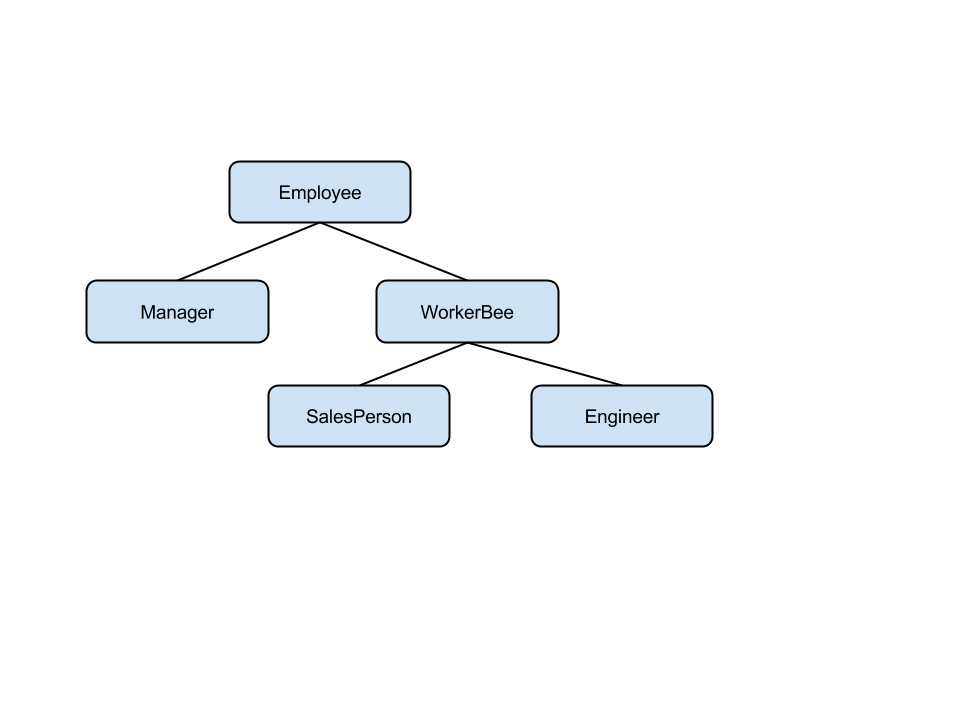
\includegraphics[width=240pt,height=180pt,keepaspectratio]{graphics/java_subclass.png}
\caption{\cite{javaObjectClass}}
\end{figure}
As you can see in this example \textit{Engineer} is an \textit{Employee}. But \textit{Manager} which also is an employee has not the same properties. 


\item \textbf{Abstract Class:}
An abstract class is a class that can't be instantiated. It's only purpose is for other classes to extend. Abstract classes are similar to Interfaces but an abstract class, in contrast, provides more structure. It usually defines some default implementations and provides some tools useful for a full implementation.\cite{javaAbstractVsInterface}

\item \textbf{Package:} 
A package is a namespace for organizing classes and interfaces. Packages make large software projects easier to manage. \cite{javaOBjectOracle}
\end{enumerate}


\subsection{Design Patterns}
Design patterns are proven solutions approaches to specific problems. A design pattern is not a framework! They are based on the base principles of object orientated design. 

\begin{enumerate}
\item Program to an interface not an implementation
\item Favor object composition over inheritance.
\end{enumerate}

\subsection{Performance}
Programs written in Java have the reputation of being slower than other languages. However in the last 10 years the JVM execution speed increased dramatically. In six separate web performance benchmarks, Java frameworks took 22 out of the 24 top-four positions. The JVM has been optimized that much that Java code is now running nearly as fast as C++ code. \cite{javaPerfromance}

\subsection{JVM}
The Java virtual machine is what makes Java a platform independent programming language. A virtual machine (VM) is a software implementation of a machine (i.e. a computer) that executes programs like a physical machine. Therefore, the JVM runs on all kinds of hardware to execute the Java Bytecode without changing the Java execution code. Java developers do not need to know how the JVM exactly works. However a deeper knowledge of the JVM helps understanding how JAVA works and can be helpful to solve various problems.\cite{javaJVM} 
\\


Features of JVM:
\begin{enumerate}
\item \textbf{Stack-based virtual machine:} Most computer architectures such as Intel x86 Architecture and ARM Architecture are based on registers. Whereas the JVM is stack based.\cite{javaJVM} That means that the VM doest need to know the operand addresses, it only calls the Stack-Pointer which points to the current instruction. \cite{stackBased_vs_registerBased} 
\item \textbf{Symbolic reference:} All data types except for primitives are referred to through a symbolic reference.   
\item \textbf{Garbage collection:} The garbage collector frees the memory from objects that are not in use any more. \cite{javaGarbageCollector}  
\item \textbf{Guarantees platform independence by clearly defining the primitive data type:} In other more tradition languages like C or C++ primitive data types have different sizes according to the System. In Java the JVM defines a fixed size for primitives. 
\end{enumerate} \cite{javaJVM}

\subsection{Java bytecode}
The Java bytecode is the result of a compiled Java source-code. It is a middle-language between Java and the machine code. \cite{javaJVM}  

\subsection{Java Code Execution Process} 
The Java code execution process is shown in the following figure. 
\begin{figure}[H]
\centering
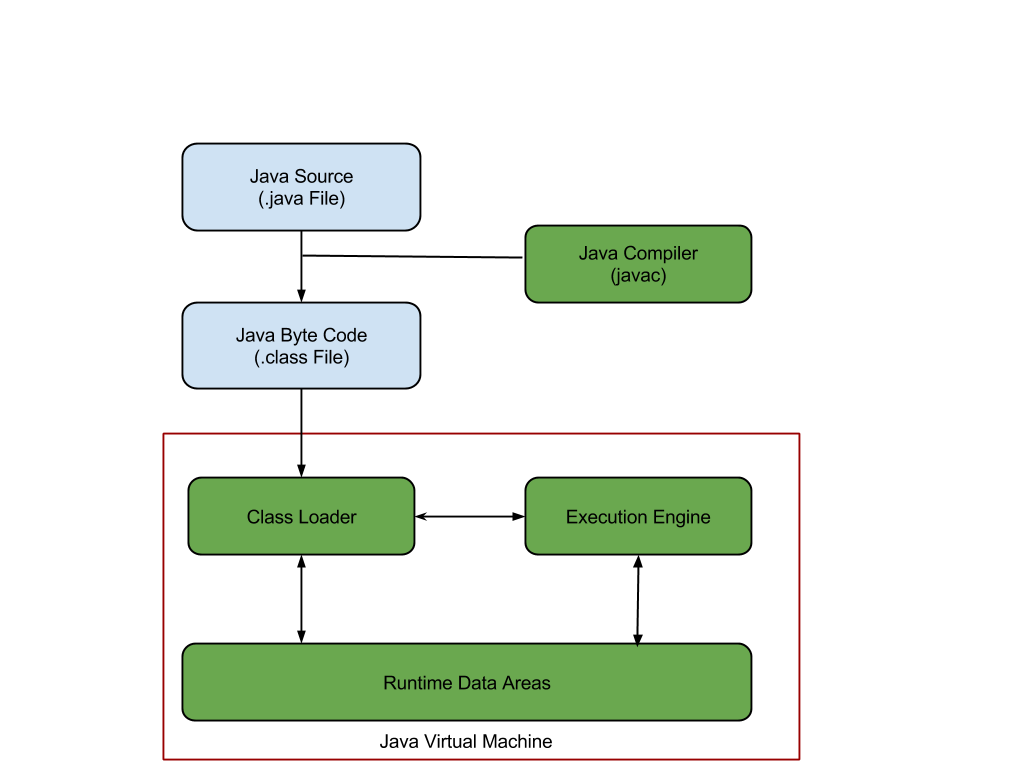
\includegraphics[width=\textwidth,height=\textheight,keepaspectratio]{graphics/java-code-execution-process.png}
\caption{java code execution process \cite{javaJVM}}
\end{figure}
\subsubsection{Class Loader}
The Java Class Loader loads and links a class when it refers to a class the first time at runtime. Every class loader has its own namespace that stores the loaded classes.\cite{javaJVM} 

\subsubsection{Runtime Data Areas}
The JVM Runtime Data Areas is the Memory assigned to a program when it runs on the OS. They can be divided into six areas: the Pc Register, JVM Stack, Native Method Stack, Heap, Method Area, and the Runtime Constant Pool. The first three are created for a single thread the other areas are shared by all threads.  

\begin{enumerate}
\item \textbf{PC register:} One \textbf{program counter} register exists for one thread. It gets created when the thread starts. Pc register has the address of the JVM instruction that is executed now.\cite{javaJVM}
 
\item \textbf{JVM Stack:} Each thread has a private JVM Stack, created the same time as the thread. A Java Virtual Machine stack stores frames. Frames are used to store data and results, new frames are created each time a method is invoked. It gets destroyed when its method invocation completes, whether that completion is normal or abrupt (it throws an uncaught exception). \cite{javaVMOracle}

\item \textbf{Native Method Stack:}
A stack for native code written in a other language than Java. It is a stack used to execute C od C++ Methods.\cite{javaJVM}.  

\item \textbf{Heap:}
The JVM Heap is a data area that is shared among all Java Threads. The heap is created on virtual machine start up.
Its a space that stores all class instances Arrays and Variables. If a program requires more heap space than aviable the Java Virtual Machine throws an \textbf{OutOfMemoryError}\cite{javaVMOracle}

\item. \textbf{Method area:} The method area is shared by all threads, created when the JVM starts. It stores runtime constant pool, field and method information, static variable, and method bytecode for each of the classes and interfaces read by the JVM. Unlike in the heap the garbage collection in the method area is optional for each JVM version. \cite{javaJVM}

\item \textbf{Runtime constant pool:}
The Runtime pool is a part of the Native Method stack and gets created when a class or interface gets created. Its the run-time representation of the \textbf{constant pool} table in a class file. This constant pool table contains several constants \cite{javaVMPaper}

For example:
\begin{lstlisting}[language=Java, caption=Java example Code]
System.out.println("Hello, world!");
\end{lstlisting}
Generated byte-code:
\begin{lstlisting}[language=Java, caption= JVM bytecode]
0:   getstatic       #2;               
3:   ldc     #3;                         
5:   invokevirtual   #4; 
\end{lstlisting}
\#n indicates that this is a reference to the constant pool.
2 is a symbolic reference to \textit{System.out}, \#3 is the \textit{Hello, world!} string.\#4 references to the \textit{PrintStream.println(String)} method.
\cite{javaVmstover}  
\end{enumerate}
\begin{figure}[H]
\centering
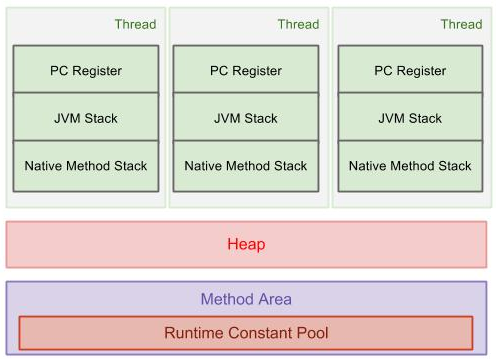
\includegraphics[width=\textwidth,height=\textheight,keepaspectratio]{graphics/java-data-areas.png}
\caption{Java Run-time Data Areas \cite{javaDataAreas}}
\end{figure}
\newpage

\subsubsection{Execution Engine}
The bytecode that is assigned to the runtime data areas in the JVM loaded from the class loader is executed by the execution engine. The execution engine reads the Java Bytecode in the unit of instructions. It is like a real CPU executing the machine commands one by one. Each command consists of 1 Operation Code byte and an additional Operand code. The execution engine gets one OpCode and execute task with the Operand, and then executes the next OpCode.\cite{javaJVM}  

\subsection{.JAR File}
A JAR \textbf{(Java ARchive)}is a file  that contains the class, image, sound, etc. files for a Java application or applet gathered into a single file and possibly compressed. \cite{javaJarMargaret}

\subsubsection{Executable JAR }
Its also possible to create a executable .Jar files. It behaves similar to a .exe file in Windows. It can be executed with a double click when Java is installed on the system. 

\section{JavaScript, HTML5,CSS3}
 \subsection{JavaScript}
 Web programing uses JavaScript. It will be used to make the web page interactive. JavaScript is very use full to change the content dynamically of a web page. It is also a expansion for HTML5 and CSS. JavaScript was developed in 1995 by Brendan Erich. JavaScript describes a dynamic typed, object oriented and classless scripting language.\cite{javascript}
 \\\\
 \subsection{HTML5}
 Html5 is the latest standard version of HTML. HTML has also previous version such as HTML 4.01, came in 1999. In that year the internet has changed significantly.HTML was created to replace  both HTML 4, XHTML and the HTML DOM Level 2. HTML5 is designed that nobody has to use extra plugins. It is capable to do such as animations to graphics, music to movies, and it can also be used to build complicated web applications. The big benefit from HTML5 is ,it is cross-.platform. It can be used for designing app for PC, Tablet, Smartphone and TV.\\\\
 HTML5 is a cooperation between the World Wide Web Consortium (W3C) and the Web Hypertext Application Technology Working Group (WHATWG).\\\\
 
  The new features of html5 is to play video and audio in a easier way. The next ability is to draw graphics. With HTML5 , web applications can be developed very easy:\\
  \begin{itemize}
  \item Local data storage
  \item Local file access
  \item Local SQL database
  \item Application cache
  \item Javascript workers
  \item XHTMLHttpRequest 2
  
  \end{itemize}
  
  Furthermore HTML5 is able to use CSS3.\cite{html5}
  \\\\
  \subsection{CSS3}
  CSS3 is the latest version of CSS. The benefit of CSS3 is, it is completely backwards-compatible with earlier version of CSS. Moreover CSS3 has been split into 'modules'. However it contains old CSS Specification, which has been split into smaller pieces .
  \\\\
  The new Modules that has been added and which are most important in CSS3 are:\\
  \begin{itemize}
  \item	Selectors
  \item	Box Model
  \item Backgrounds and Borders
  \item	Image Values and Replaced Content
  \item	Text Effects
  \item	2D/3D Transformations
  \item	Animations 
  \item 	Multiple Column Layout
  \item User Interfaces
  
  \end{itemize}
  \cite{CSS3}
  \\\\
  \section{jQuery Mobile}
  jQuery Mobile is Touch-Optimized Web Framework. This Framework was created by the JQuery Foundation. It is completely open source. This Framework is also one of the most popular Mobile frameworks. That's the  reason why this project NAVAR uses JQuery Mobile Framework. This Framework was created by Jasper de Groot, Alexander Schmitz, Anne-Gaelle Colom, Gabriel Schulhof.\\\\
  
  jQuery Mobile is a HTML5 based user interface system, it is designed to create responsive web sites and apps that are accessible on all smartphones, tablets and desktop devices. The Framework is build on jQuery and jQuery UI foundation. It offers also Ajax navigation with page transitions, touch events and it has other interesting components and features. This Module is a lightweight code, so it has a flexible ,easily theme able design. \\\\
  
  jQuery Mobile  also updates their Framework versions. To built a Theme with the Framework is not so difficult. The User interface has the components of jQuery Mobile. The components of jQuery will be explained in Chapter X.\\\\
  
  \section {AJAX}
  AJAX (Asynchronous JavaScript and XML) is a method which is widely used in web development. Ajax uses several technologies like: JavaScript, CSS, XML and XMLHttpRequest.\cite{ajax}
  \\
  \subsection{XML}
  \textit{''Extensible Markup Language (XML) is a simple, very flexible text format derived from SGML (ISO 8879). Originally designed to meet the challenges of large-scale electronic publishing, XML is also playing an increasingly important role in the exchange of a wide variety of data on the Web and elsewhere.''}\cite{xml}
  \\
  \subsection{XMLHttpRequest}
  XMLHttpRequest is used in Ajax for exchanging data with a server. The main advantages of this request is that it can be used in the background for sending data to the server, updating a page without reloading it, request and receive data from the server after the page is loaded.\cite{xmlHttp} 
  \newpage
  \subsection{How does AJAX work?}
  \begin{figure}[htbp]
  \centering
  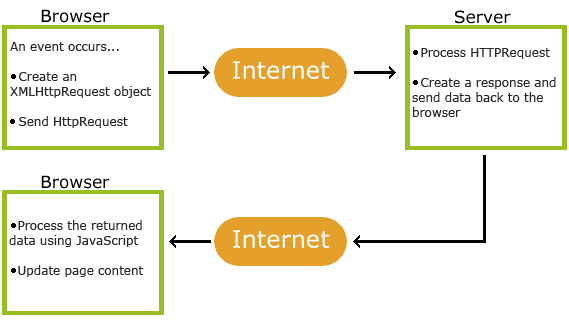
\includegraphics[width=100mm,height=\textheight,keepaspectratio]{graphics/ajaxwork.png}
  \caption{AJAX overview\cite{ajax}}
  \end{figure}
  
  As described in the graphic, whenever a program needs to send data from the browser to the server it creates an XMLHTTPRequest object. This request is then accepted or denied by the server and a response will be sent back to the browser where it can be displayed or processed. 
  
  \section{Windows Azure}
  \textit{''Azure is an open and flexible cloud platform that enables you to quickly build, deploy and manage applications across a global network of Microsoft-managed datacenters. You can build applications using any language, tool or framework. And you can integrate your public cloud applications with your existing IT environment''}\cite{azure}
  \subsection{Overview}
  \begin{figure}[htbp]
  \centering
  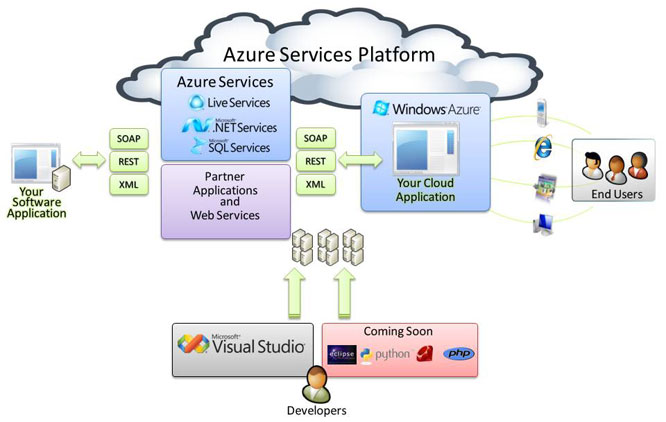
\includegraphics[width=100mm,height=\textheight,keepaspectratio]{graphics/azurePlattform.jpg}
  \caption{Azure overview}\cite{azureOver}
  \end{figure}
  
  The typical Windows Azure environment consists of many components such as the Azure Service Platform, which can be several virtual machines with services. A software application which communicate with Azure over XML and other technologies. Several end users which access the Azure cloud over a browser and developers who access the cloud directly. 
  \newpage
  \section{Microsoft SQL Server}
  Microsoft SQL Server is a relation database software for saving,modifying and providing data. Microsoft SQL Server can be deployed on a desktop server as well as in the cloud.It provides a edition for high-end performanc, critical applications and a lighter version for normal applications/data.\cite{sqlserver}
  \\\\
  There are five main releases of MS SQL Server:
  \begin{itemize}
          \item Microsoft SQL Server 2005
          \item Microsoft SQL Server 2008 
          \item Microsoft SQL Server 2012 
          \item Microsoft SQL Server 2014
  \end{itemize}
        \cite{sqlserver}
  \subsection{Program Overview}
  \begin{figure}[H]
  \centering
  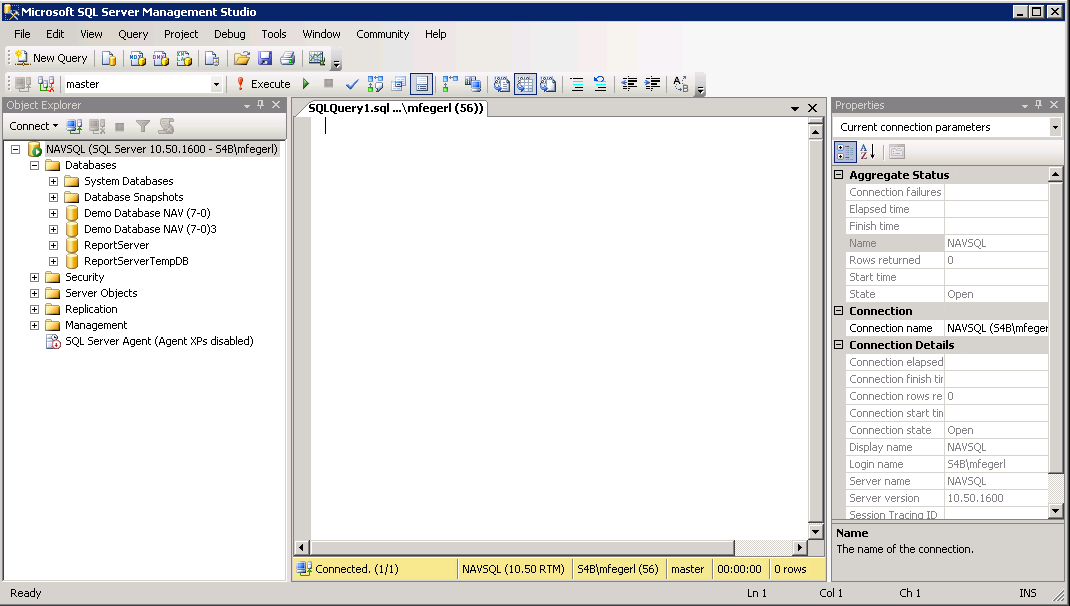
\includegraphics[width=\textwidth,height=\textheight,keepaspectratio]{graphics/sqlserver.png}
  \caption{SQl Server 2008 overview}
  \end{figure} 

  The figure shows the graphical user interface of  Microsoft SQL Server Management Studio. It is used to maintain and configure SQL databases. In the left panel of the program the available databases are shown.The panel in the middle is a simple editor for database queries.On the right side the properties of the selected datbase are displayed.    
  \newpage
  \section{Microsoft Dynamics NAV}
  Microsoft Dynamics NAV is an ERP(Enterprise Ressource Planing) software for small and medium sized corporations. It is a highly adaptable software which provides functionalities for managing a whole business. Such as sales, shipping, financing, project management, supply chain management, business intelligence,reporting and other services. 
  The look and feel of the application is based on Microsoft Office to provide a simple entry point to the product if you are familiar with Microsoft Office. Microsoft NAV can be either installed on local servers as a 3-tier ,2-tier or 1-tier implementation as well as in the cloud to provide the best solution for a business.\cite{navOver} 
  
  \subsection{Program Overview}
  The following figure shows the graphical user interface of Microsoft NAV, the RoleTailored client(RTC).It shows the RTC for the role sales manager with the demo Database ''CRONUS International Ltd.'' from Microsoft. 
  \begin{figure}[htbp]
  \centering
  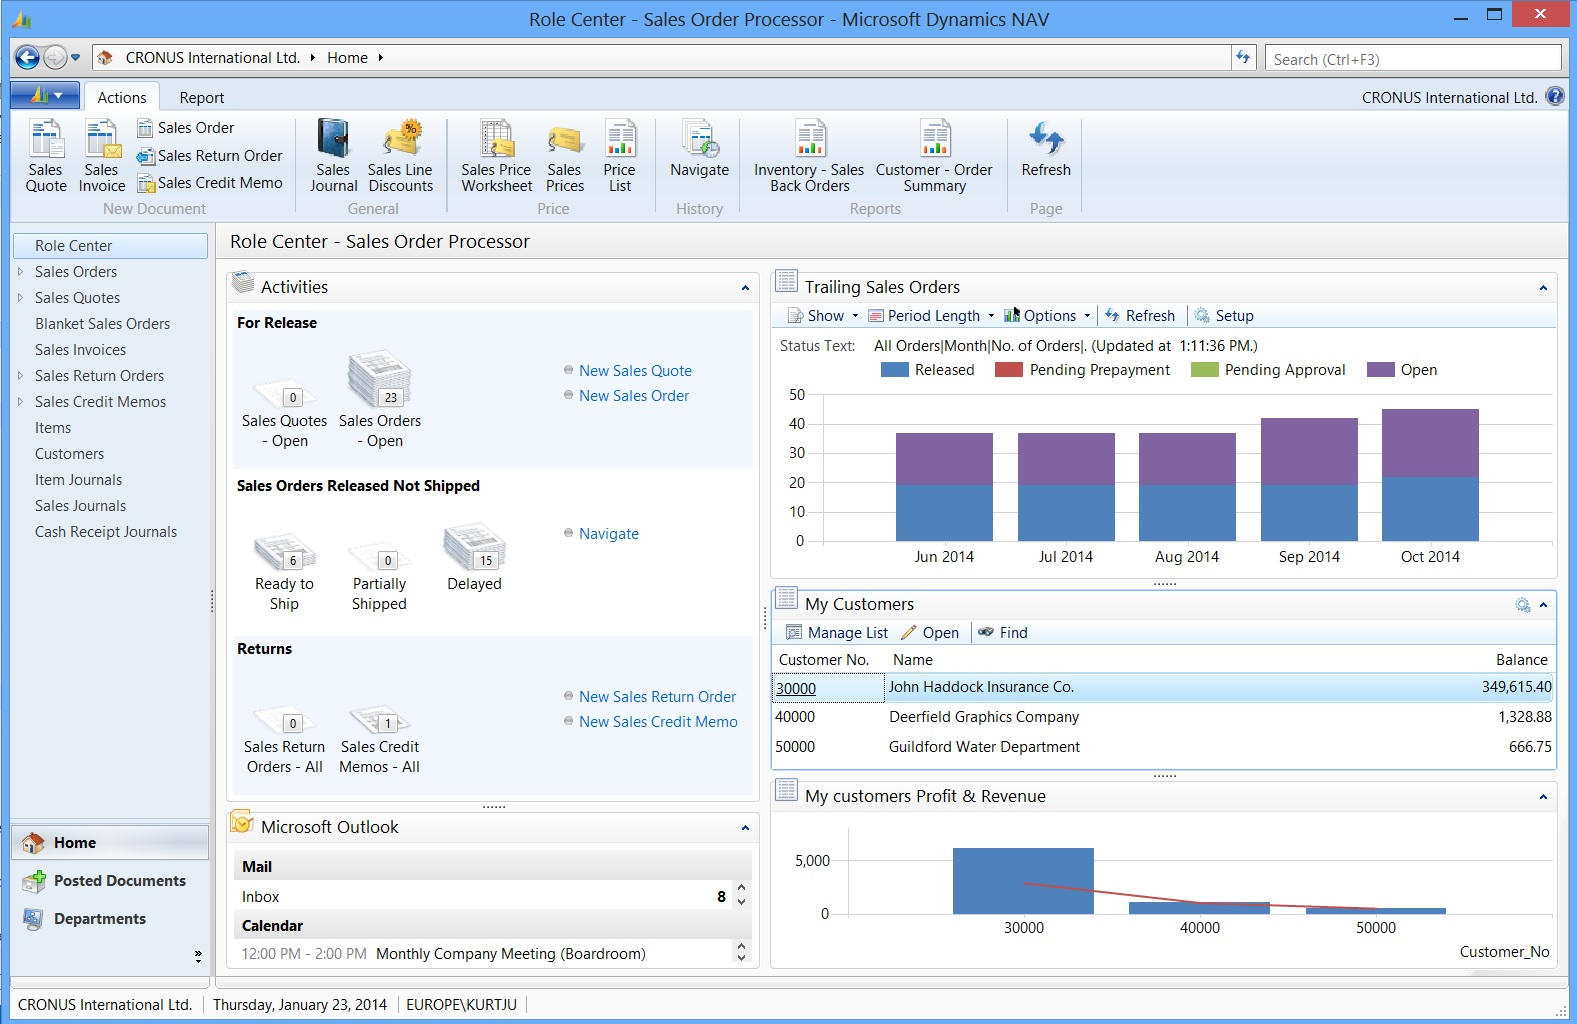
\includegraphics[width=\textwidth,height=\textheight,keepaspectratio]{graphics/navSales.jpg}
  \caption{Program overview}\cite{azureOver}
  \end{figure}
  \newpage
  
  \subsection{Data structure}
  \subsubsection{Tables}
  Microsoft Dynamics NAV saves data into a Microsoft SQL Server database.The databases consist of several tables, which can be created, edited and deleted.\\Table's are the basic modules of the database and are fundamental.It provides the functionality to modify,delete and display data on the run.
  \\\\
  \begin{figure}[htbp]
  \centering
  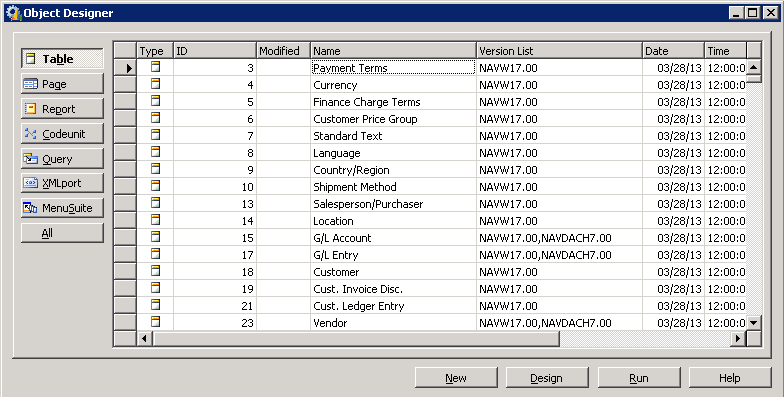
\includegraphics[width=\textwidth,height=\textheight,keepaspectratio]{graphics/navTable.png}
  \caption{Table example}
  \end{figure}
  \newpage
  \subsubsection{Pages}
  A page is a XML object which consists of several properties and code. It is used to display, structure and organize data. It can either be accessed via a client and displayed graphically or trough a web service.In this project the pages are used over a web service by the C\# application. The usage of the pages are explained in the chapter ''Streaming''. 
  \\\\
  The following figure shows an example page with a list of customers.
  \begin{figure}[htbp]
  \centering
  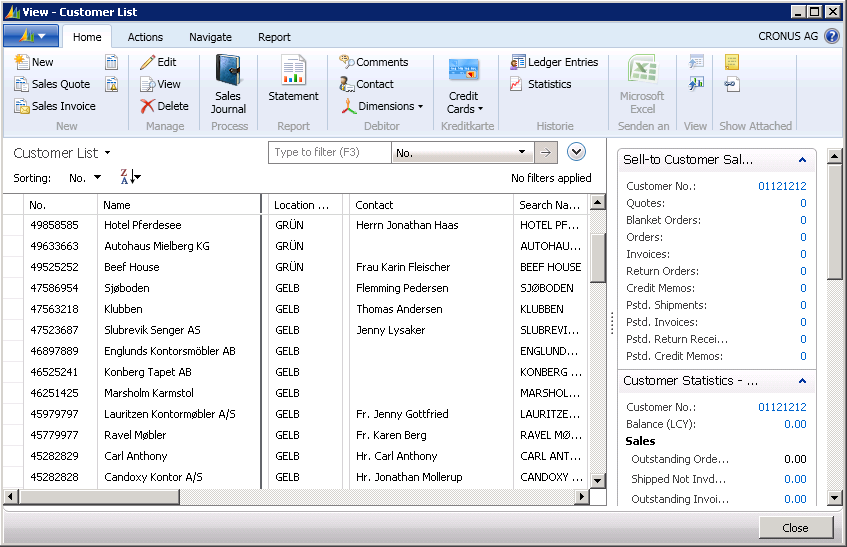
\includegraphics[width=\textwidth,height=\textheight,keepaspectratio]{graphics/customerlist.png}
  \caption{customer page example}
  \end{figure}
  \newline
  This page displays the content of the table customers.
  It consist of several attributes such as the name and the telephone number of a specific person.The page provides the functionality to create, delete or  modify the customers within the RTC.    
 
%
\chapter{Integrated Development Environment}


%George, Pokorny
\section{Andorid SDK Eclipse}




















%Korabach
\section{JetBrains WebStorm}
The application’s logic had to be created with a programming language called JavaScript. Because of that, the project group had to find a development environment that’s best suited for this language. JetBrains WebStorm 7.0.3 was best fit for all future tasks and should be the environment in which JavaScript had been developed. 
\\

However, not only JavaScript, but also HTML as well as CSS could be developed with this IDE. All information about this product can be found on Jet Brains homepage.\cite{webstorm}
\subsection{Overview}
JetBrains WebStorm is a professional JavaScript IDE that supports a wide range of modern technologies related to JavaScript programming language, HTML and  CSS, and provides the complete experience for productive Web development.
\\

WebStorm offers developers an intelligent code editor that truly supports the structure of code written in JavaScript, HTML or CSS, as well as their modern  successors. It features the best-of-breed coding assistance for a whole set of  cutting-edge web technologies, including code completion, refactorings, code formatting, on-the-fly error prevention, and much more. 
\\

WebStorm is also great for developing Node.js applications. Together with integrated instruments 
for testing, debugging and code analysis and integration with various VCS, WebStorm is an essential tool for powerful and productive web development.
\\

\begin{figure}[h]
\centering
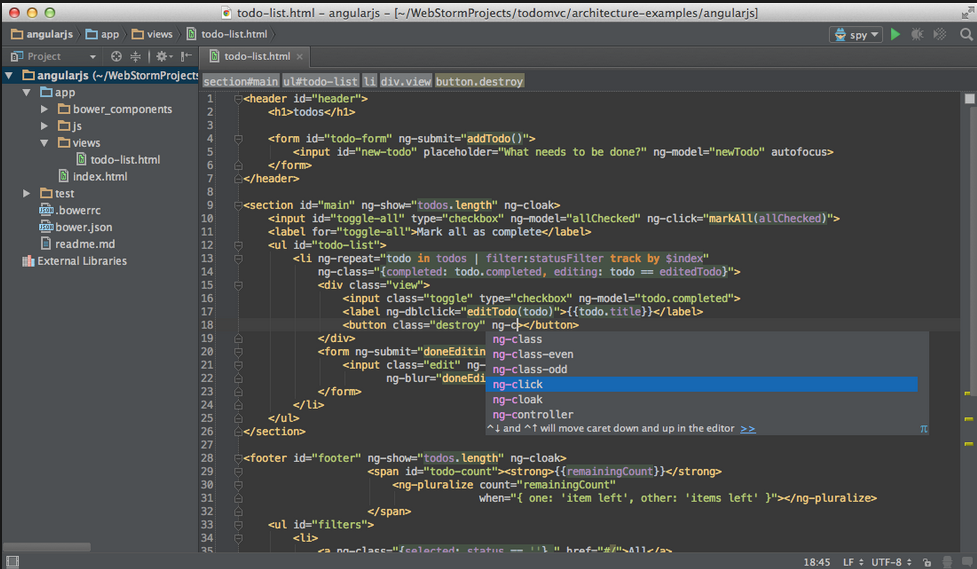
\includegraphics[width=1\linewidth]{graphics/chapter3/1}
\caption{WebStorm Interface}
\label{}
\end{figure}


\subsection{Features}
\begin{itemize}
\item Intelligent JavaScript, HTML, and CSS editor with syntax highlighting, code completion, configurable formatting configuration, refactorings, on-the-fly error detection and support of language mixtures.
\item Support for a wide range of technologies: TypeScript, CoffeeScript, Dart, LESS, Sass, Stylus, Compass, EJS, Handlebars, Mustache, Web Components, Jade, Emmet, and many more.
\item Productivity-boosting Live Edit feature: See the changes in the browser immediately without reloading the page.
\item 
JavaScript debugger for Chrome and Firefox, with breakpoints, stepping, frames view and watchers. Full-featured debugging of TypeScript, CoffeeScript and Dart with sourcemaps.
\item 
File Watchers for automatic compilation/transpilation of higher-level languages like TypeScript, CoffeeScript, LESS, Sass, and Stylus.
\item 
A debugger for Node.js applications with the latest features of V8 Debugger Protocol.
\item 
Intelligent code inspections, one-click quick-fix suggestions, JSHint, JSLint, and Google Closure Linter.
\item
JavaScript unit testing with integrated JSTestDriver or Karma test runner with code coverage. 
\item
Built-in HTTP Server, REST Client, Terminal and Node.js package manager npm. 
\item 
New Project Wizard with well-known project templates like Twitter Bootstrap and Node.js Express App.
\item
Integration with Version Control Systems including Git, Subversion, Mercurial, CVS, Perforce, and GitHub. 
\item 
Easily configurable FTP/FTPS/SFTP deployment.
\item 
Integration with various issue trackers.
\end{itemize}
















%Fegerl
\section{Visual Studio}

%
\chapter{Implementation in JavaScript} \label{chapter:desgin}

The logic of this app is divided into two parts. First part is JavaScript logic, that is responsible for the functionalities of each HTML site, more precisely, the dynamic response to the user. Second part is Java Android logic, which is responsible for the main function called car tracking and all other functionalities that could not be accomplished with help of JS. 
\\

Altogether there are 10 HTML sites and each one of them has some functionalities that had to be implemented with JS or Android Java. A simple example of a functionality is pressing a button. This button triggers a function inside the JS. 
\\

However, JavaScript and Android Java did not provide everything that has been needed for the project application. That's the reason why project members had to use several other web frameworks like jQuery or phonegap.js. This was necessary to accomplish the main goal of a powerful, user-friendly mobile application. The usage of web frameworks will be explained in following chapters. 
\newpage



\section{Display}
This chapter describes the functionality behind each display of mobile application. 


\subsection{Start Menu}
The Start menu is displayed after the application was started. It provides user with several functions like help, car tracking, favourite list, about and exit. Basically it is the first thing that user sees and from there he navigates threw the whole application.
\\

\begin{figure}[h]
\centering
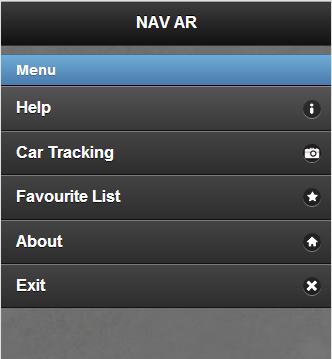
\includegraphics[width=0.5\linewidth]{graphics/chapter4/1}
\caption{Start menu}
\end{figure}


Each one of these buttons have their logic that is implemented in \textbf{index.html}.
\newpage The listing 4.1 shows the functionality behind each button.
\\

\begin{lstlisting}[language=html, caption= 
Start menu source code,captionpos=b]
<li data-icon="info">
  <a href="help.html" rel="external">
    Help
  </a>
</li>
<li data-icon="camera">
  <a href="#" onclick="trackClick();">
    Car Tracking
  </a>
</li>
<li data-icon="star">
  <a href="myfavourite.html" rel="external">
    Favourite List
  </a>
</li>
<li data-icon="home">
  <a href="about.html" rel="external">
    About
  </a>
</li>
<li data-icon="delete">
  <a href="#" onclick="turnOff();">
    Exit
  </a>
</li>
\end{lstlisting}


\
\
Functions \textit{trackClick()} and \textit{turnOff()} were implemented in Android Java and are described in chapter 5)''Implementation in Android Java and Metaio Tracking''.
\\


\begin{lstlisting}[language=html, caption= 
JavaScript functions in start menu,captionpos=b]
function trackClick() {
    MyTracking.performClick();
}

function turnOff(){
	Exit.exitClick();
}
\end{lstlisting}


The button \textbf{help} forwards the user to the help display \textit{help.html}. The same functionality features \textbf{about} and \textbf{favourite list}, except they link to another display. 
\\

\textbf{Exit} button invokes the function \textit{turnOff()} which calls another Android Java implemented function. \textit{Exit.exitClick()} ends the application. Illustrated in listing 4.2.
\\

\textbf{Car tracking} calls a function \textit{trackClick()}. This method starts the main function.
\\
\newpage


\subsection{Help}
The help display provides only two major options: back button and the link to a tutorial video. This tutorial was created by the project members and is an YouTube video.


\begin{figure}[h]
\centering
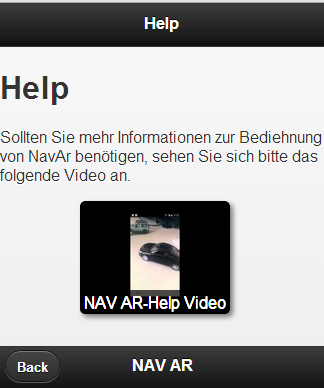
\includegraphics[width=0.5\linewidth]{graphics/chapter4/2}
\caption{Help display}
\end{figure}


The back button leads to the main menu. Shown in listing 4.3.
\\
\begin{lstlisting}[language=html, caption= 
Back button,captionpos=b]
<a class="ui-btn-left" href="index.html" rel="external">
	Back
</a>
\end{lstlisting}
\
\


If the user touches the picture \textbf{NAV AR - Help Video}, he will be linked to a specific how-to YouTube video. This video serves as a simple help to understand how the application works. It shows how to use the application's main functions and more.
\\

\begin{lstlisting}[language=html, caption= 
Help video,captionpos=b]
<a href="https://www.youtube.com/watch?v=6U4oT5AbAsre">
  NAV AR-Help Video
</a>
\end{lstlisting}


%%%%%%%%%%%%%%%%%%%%%%%%%%%%%%%%%%%%%%%%%%%%%%%%%%%%%%%%%%%%%%%%%%
%New Chapter Main Menu
%%%%%%%%%%%%%%%%%%%%%%%%%%%%%%%%%%%%%%%%%%%%%%%%%%%%%%%%%%%%%%%%%
\subsection{Main Menu}
The most important function of the whole mobile applications is \textbf{car tracking}. This function is executed by \textit{MyTracking.peformClick()}. More in chapter 4.1)''Start Menu''.
\\

After a car was successfully tracked, the user is linked to a new display called \textbf{index.html}, which is the start menu. It provides the user with additional options. Options that deliver technical information as well as review about the tracked car and more other useful functions. 
\\

There is also a possibly to add the tracked car to users car collection named \textbf{the favourite list}. Out of there he can select one specific vehicle to use the start menu options, like picture or videos gallery.
\\

JavaScript functions had to be created for each  of this options. These functions are described in chapter 4.3.1)''JavaScript Functions''.
\\

\begin{figure}[h]
\centering
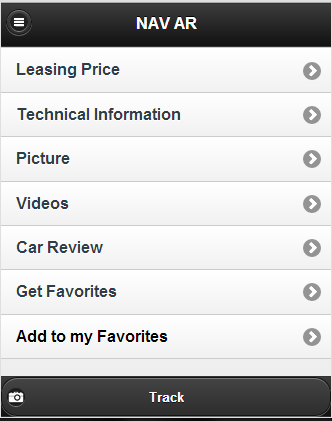
\includegraphics[width=0.5\linewidth]{graphics/chapter4/3}
\caption{Main Menu}
\end{figure}
\newpage


\
Listing 4.23 shows the function behind each button. Some buttons only link to another, other invoke specific functions like \textit{LocalStorageWriteId()}.\\
\begin{lstlisting}[language=html, caption= 
Main menu source code,captionpos=b]	
<li>
  <a href="leasingprice.html" rel="external">
    Leasing Price
  </a>
</li>
<li>
  <a href="technicalinfo.html" rel="external">
    Technical Information
  </a>
</li>
<li>
  <a href="slide.html" rel="external">
    Picture
  </a>
</li>
<li>
  <a href="video.html" rel="external">
    Videos
  </a>
</li>
<li>
  <a href="#" rel="#" onclick="reviewClick();">
    Car Review
  </a>
</li>
<li>
  <a href="myfavourite.html"rel="external">
    Get Favorites
  </a>
</li>
<li>
  <a id="add_favorite" 
  onclick="LocalStorageWriteId
  (sessionStorage.getItem('id'),globalcarname);"
   style="color:red" rel="external">
     Add to my Favorites
  </a>
</li>
\end{lstlisting}
\newpage


\subsubsection{Leasing Price}
%%%%%%%%%%%%%%%%%%%%%%%%%%%%%%%%%%%%%%%%%%%%%%%%%%%%%%%%%%%%%%%%%%%%
%link to chapter with leasing price technologie
%%%%%%%%%%%%%%%%%%%%%%%%%%%%%%%%%%%%%%%%%%%%%%%%%%%%%%%%%%%%%%%%%%%%
When the user presses on button \textbf{leasing price} he will be linked to the html page \textit{leasingprice.html} where he receives informations about the specific vehicle. \\
\
\

\begin{figure}[h]
\centering
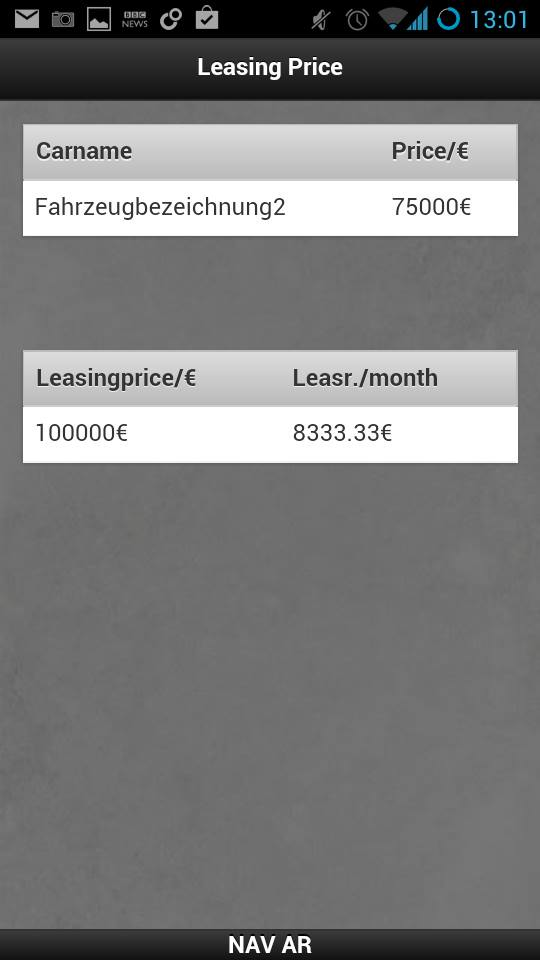
\includegraphics[width=0.5\linewidth]{graphics/chapter4/5}
\caption{Leasing Price}
\end{figure}
\newpage


\subsubsection{Technical Information}
By calling \textbf{technical information} facts about a specific car are presented. To create it several new features had to be used. Phone Gallary and Dynamic Selection of Colour. Informations about those are featured in chapters 4.6)''Photo Gallery'' and  4.8)''Dynamic Selection of Colours''.
\\

\begin{figure}[h]
\centering
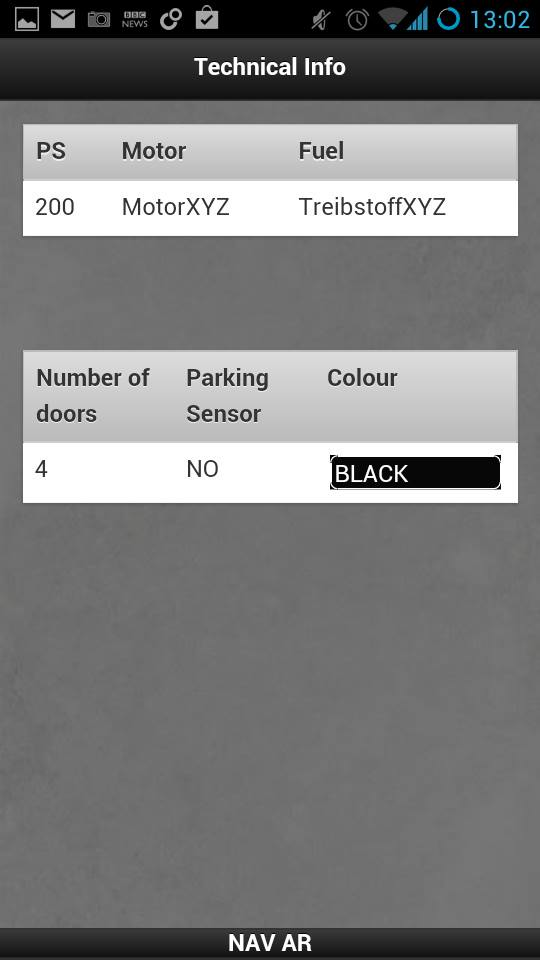
\includegraphics[width=0.5\linewidth]{graphics/chapter4/6}
\caption{Technical Information}
\end{figure}
\newpage

\subsubsection{Pictures}
Has freshest pictures of the specific car. Feature called Photo Gallery in chapter ..... was used to create this option.

\begin{figure}[h]
\centering
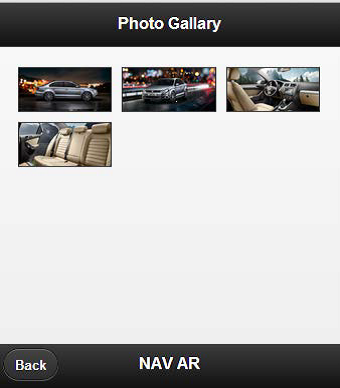
\includegraphics[width=0.5\linewidth]{graphics/chapter4/7}
\caption{Pictures}
\end{figure}
\newpage

\subsubsection{Videos}
This option provides the user with videos about the selected car from favourite list or fresh tracked one. More about video gallery in chapter.....
\\
\begin{figure}[h]
\centering
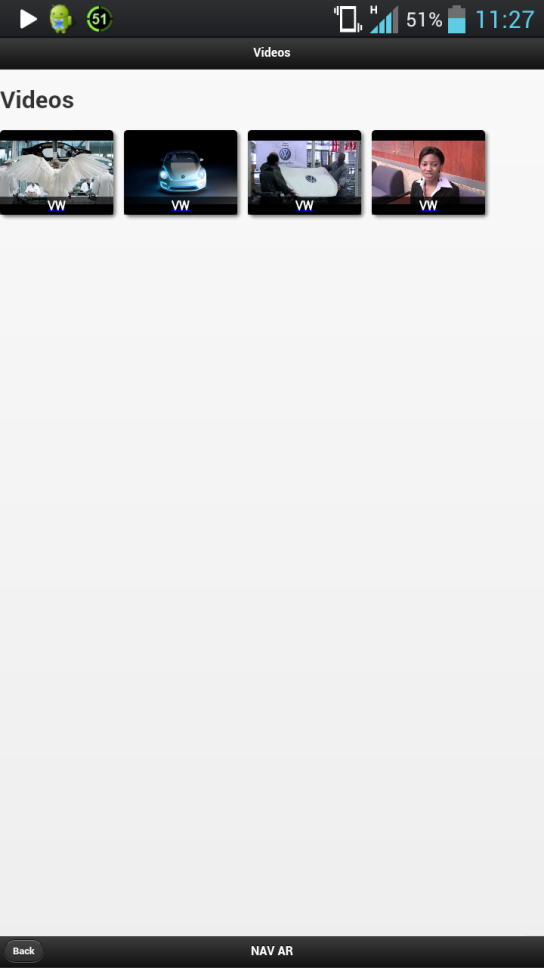
\includegraphics[width=0.5\linewidth]{graphics/chapter4/8}
\caption{Video Gallery}
\end{figure}
\newpage

\subsubsection{Review}
Operation review invokes a self created method called \textit{reviewClick()}. Description to thisit is in chapter 4.3.1 Created Methods, Review. Basically review links the user to a new display where he can read review about the specific car.
\\

\begin{figure}[h]
\centering
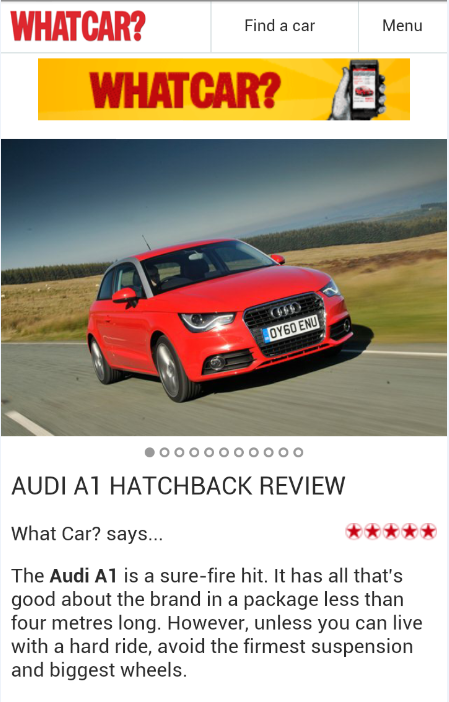
\includegraphics[width=0.5\linewidth]{graphics/chapter4/9}
\caption{Review}
\end{figure}
\newpage


\subsubsection{Get Favourites}
This operations links the user to his favourite cars which he saved with the option \textbf{add to my favourite}. Information about the favourite list in chapter 4.4)My Favourites.
\\

\begin{figure}[h]
\centering
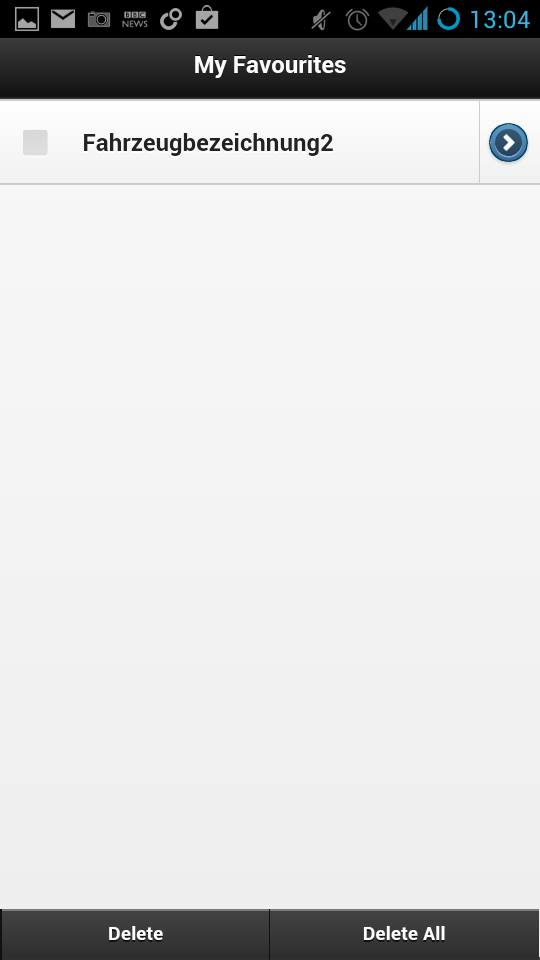
\includegraphics[width=0.5\linewidth]{graphics/chapter4/10}
\caption{Favourite list}
\end{figure}
\newpage

\subsubsection{Add to my Favourites}
The button \textbf{Add to my Favourites} trigger the function \textit{LocalStorageWriteId()}. It saves the id and the name of the tracked car into users favourites. For the first parameter it takes the tracked car id from the session storage. For the second parameter the global variable \textit{globalcarname}.
\\

\begin{lstlisting}[language=html, caption= 
add favourite sorce code,captionpos=b]
<li>
  <a id="add_favorite"onclick="LocalStorageWriteId
  (sessionStorage.getItem('id'),globalcarname);"
  style="color:red" rel="external">
    Add to my Favorites
   </a>
</li>
\end{lstlisting}
\

\
Before the user can add the vehicle to his favourites he has to wait several seconds. In this time the request is send to the server for information about the car threw its id. If the user wants to access the operation in its loading time, the application denies him the access and informs him about the loading time.
\\

\begin{figure}[h]
\centering

\includegraphics[width=0.65\linewidth]{graphics/chapter4/11}
\caption{Not ready function}
\end{figure}
\

The operations colour changes from red to black when the function is loaded.
\\
\begin{figure}[h]
\centering

\includegraphics[width=0.65\linewidth]{graphics/chapter4/12}
\caption{Ready function}
\end{figure}
\newpage

\subsection{My Favourites}
Inside the favourites are cars had been added threw the operation \textbf{add to my favourites}. The favourite cars can be selected or deleted. Removing the cars from favourites is possible by selecting the specific vehicle or removing all of the cars.
\\

\begin{figure}[h]
\centering
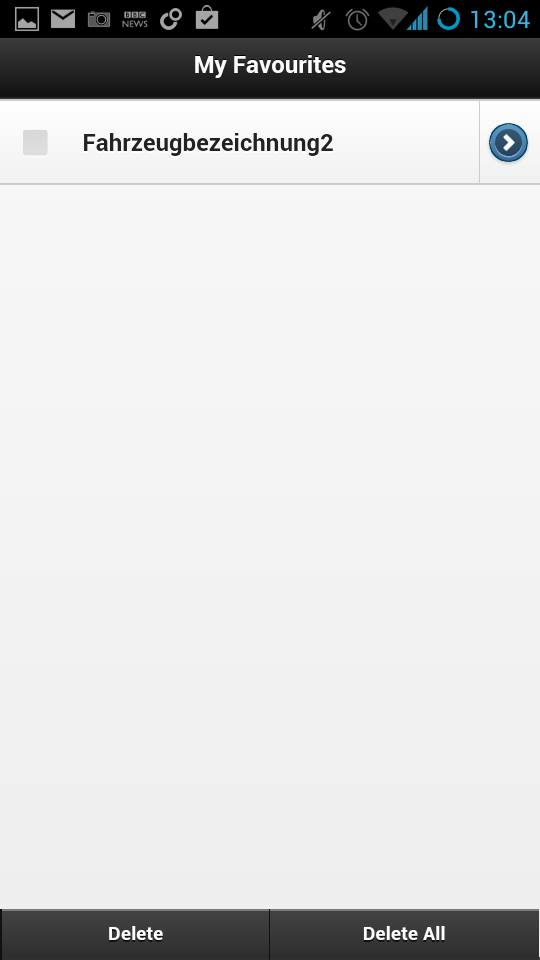
\includegraphics[width=0.4\linewidth]{graphics/chapter4/15}
\caption{My Favourites display}
\end{figure}
\



\subsubsection{Loading of favourite cars}
Before the functions of the favourite list can be used, the list entries(cars) have to be initialized. This is done automatically when the site is loaded. 
\\

Each line that is written inside document.ready starts after the document is ready. This is where the favourite cars are initialized.
\\
\newline
\newline

\begin{lstlisting}[language=html, caption= 
source for document is ready,captionpos=b]
$(document).ready(function () {
.
});
\end{lstlisting}
\

First, all car names are loaded from local storage into an array called \textit{storedCarNames}. So this array is filled with vehicle names which user added to his favourites. 
\\

\begin{lstlisting}[language=html, caption= 
Array with favourite cars,captionpos=b]
var storedCarNames = JSON.parse(localStorage["fcarname"]); 
\end{lstlisting}
\


Now the filling of the cars into a list begins. The loop goes so long as the number of cars in the array. In this loop a car name is put into the \textit{listItem1} which is just a panel shown in figure 4.17.
\\

Next \textit{listItem1} is put into another list. This list is where all panels(favourite cars) are stored. Each new vehicle is put into the list.
\\
\begin{lstlisting}[language=html, caption= 
Adding list items into the list,captionpos=b]
for (var i = 0; i < storedCarNames.length; i++){
  var key = storedCarNames[i];
  listItem1 = '"specific list item"';

  $('#liste').append(listItem1);
}
\end{lstlisting}

\begin{figure}[h]
\centering

\includegraphics[width=0.7\linewidth]{graphics/chapter4/16}
\caption{A list item}
\end{figure}

Last but not least the list that has to be refreshed so the list items are displayed. 
\\

\begin{lstlisting}[language=html, caption= 
Refreshing the list,captionpos=b]
$('#liste').listview('refresh').trigger('create'); 
\end{lstlisting}


\subsection{About}
The \textbf{about} display has no logic and no self made functions except one the back button which functionality you have learnt in 4.2)Help chapter.
\\
\begin{figure}[h]
\centering
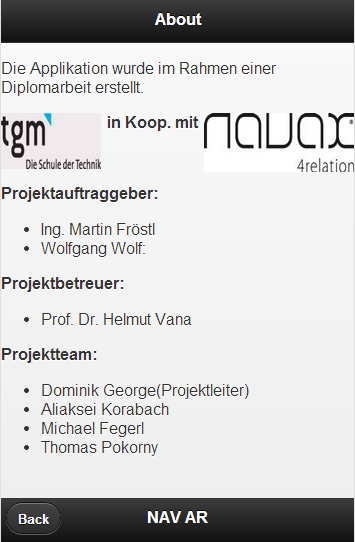
\includegraphics[width=0.4\linewidth]{graphics/chapter4/17}
\caption{About display}
\end{figure}
\newpage


\section{Implemented Function}


\subsection{Start timer}
When the site is loaded a timer automatically starts. Specific functions stop the timer and sends the time stamp to the NAV server.
\\
\begin{lstlisting}[language=html, caption= 
Start timer function,captionpos=b]
function startTime(){
	var d = new Date();
	timestart = d.getTime();
}
\end{lstlisting}

\subsection{End timer}
This function stops the timer which had been started with the method \textit{startTime()} and safes the time with the method \textit{timestampsave()}. The timer was used to get the time how long a user has selected a specific car and used certain start menu options.
\\

\begin{lstlisting}[language=html, caption= 
End timer function,captionpos=b]
function endtime(){
	var d = new Date();
	var endtime = d.getTime();
	timestampsave(timestart,endtime);
}
\end{lstlisting}


\subsection{Save the time}
This function saves start time and end time of the timer, into the NAV server. The start time and end time are the input parameters. 
\\

%%%%%%%%%%%%%%%%%%%%%%%%%%%%%%%%%%%%%%%%%%%%%%%%%%%%%%%%%%%%%%%%%%
%link to michaels chapter about the connection
%%%%%%%%%%%%%%%%%%%%%%%%%%%%%%%%%%%%%%%%%%%%%%%%%%%%%%%%%%%%%%%%%%

To save the time into the server \textit{timestampsave()} needs several other information like email and id of the tracked car. More about sending information to the server and  to the connectivity between application and server read the chapter 7.0.3.4)''Communication from mobile device to the C App''.
\\

time1.....start time
\\
time2.....end time\\
\newline


\begin{lstlisting}[language=html, caption= 
Save time function,captionpos=b]
function timestampsave(time1,time2){
  var stime	= time1;
  var endtime = time2;
  var emailan = sessionStorage.getItem('email');
  var fid = sessionStorage.getItem('id');
    
  $(document).ready(function () {
     $.ajax({
        type: "GET",
        url: "URL",
        async: false,
        dataType: 'JSONP',
        success: function(data){
        //do your stuff with the JSON data
          var test=data;
          console.log(test);
        }
     });
  });
}
\end{lstlisting}


\subsection{Set parameters}
There are two parameters that have to be saved into the session storage to establish a connection with the NAV server. That were id of the tracked car and the email address of the user.
\\
\begin{lstlisting}[language=html, caption= 
Set parameter function,captionpos=b]
function setParam(){
	window.sessionStorage.setItem('id', myVariable);
	window.sessionStorage.setItem('email',email);
}
\end{lstlisting}

%%%%%%%%%%%%%%%%%%%%%%%%%%%%%%%%%%%%%%%%%%%%%%%%%%%%%%%%%%%%%%%%%%
%link to chapter with car tracking in java android
%%%%%%%%%%%%%%%%%%%%%%%%%%%%%%%%%%%%%%%%%%%%%%%%%%%%%%%%%%%%%%%%%%
\subsection{Start car tracking}
This function starts to track a car. For more explanation refer to chapter 5)'Implementation in Android Java and Metaio Tracking'.
\\
\newline
\newline
\begin{lstlisting}[language=html, caption= 
Car tracking function,captionpos=b]
function trackClick() {
  MyTracking.performClick();
}
\end{lstlisting}

%%%%%%%%%%%%%%%%%%%%%%%%%%%%%%%%%%%%%%%%%%%%%%%%%%%%%%%%%%%%%%%%%
%link to chapter with the revie in android java
%%%%%%%%%%%%%%%%%%%%%%%%%%%%%%%%%%%%%%%%%%%%%%%%%%%%%%%%%%%%%%%%%
\subsection{Review}
This method is implemented with Java Android. More about in chapter 5)'Implementation in Android Java and Metaio Tracking'.
\\

\begin{lstlisting}[language=html, caption= 
Review function,captionpos=b]
function reviewClick(){
        Review.performClick();
    }
\end{lstlisting}

%%%%%%%%%%%%%%%%%%%%%%%%%%%%%%%%%%%%%%%%%%%%%%%%%%%%%%%%%%%%%%%%%
%link to chapter java android implementation
%%%%%%%%%%%%%%%%%%%%%%%%%%%%%%%%%%%%%%%%%%%%%%%%%%%%%%%%%%%%%%%%%
\subsection{Turn off}
This function is implemented with Android Java and has been documented in 4.1)''Start Menu''.
\\

\begin{lstlisting}[language=html, caption= 
Turn off funtion,captionpos=b]
function turnOff(){
        Exit.performClick();
    }
\end{lstlisting}


\subsection{Home}
This function returns the user back to the start menu and is implemented with Android Java.\\

\begin{lstlisting}[language=html, caption= 
Home function,captionpos=b]
function home(){
        Home.performClick();
    }
\end{lstlisting}


\subsection{Read car name}
This method returns the name of the car that had been tracked threw a car specific id. Each transport has its own unique id. This id is predefined and set after the tracking was successful. Later it is stored in session storage.
\\
\newline  
%%%%%%%%%%%%%%%%%%%%%%%%%%%%%%%%%%%%%%%%%%%%%%%%%%%%%%%%%%%%%%%%%%
%link to chapter with ajax
%%%%%%%%%%%%%%%%%%%%%%%%%%%%%%%%%%%%%%%%%%%%%%%%%%%%%%%%%%%%%%%%%%
So the input parameter \textit{cname} is that specific id of the tracked or selected car. The name of the car is stored in the NAV server. A request had to be send to receive the name. More about Connectivity in chapter 7)''Streaming''.
\\

%%%%%%%%%%%%%%%%%%%%%%%%%%%%%%%%%%%%%%%%%%%%%%%%%%%%%%%%%%%%%%%%%%
%set code on one line
%%%%%%%%%%%%%%%%%%%%%%%%%%%%%%%%%%%%%%%%%%%%%%%%%%%%%%%%%%%%%%%%%%

\begin{lstlisting}[language=html, caption= 
Read car name function,captionpos=b]
function readcarname(cname){
  var test = '';
  $(document).ready(function () {
    $.ajax({
      type: "GET",
        url:"URL",
        async: false,
        dataType: 'JSONP',
        success: function(data){
          test=data.split(';');
          globalcarname=test[0];
          document.getElementById("add_favorite").
          style.color="black";
        }
    });
  });
}
\end{lstlisting}

%%%%%%%%%%%%%%%%%%%%%%%%%%%%%%%%%%%%%%%%%%%%%%%%%%%%%%%%%%%%%%%%%%
%link to chapter with ajax
%%%%%%%%%%%%%%%%%%%%%%%%%%%%%%%%%%%%%%%%%%%%%%%%%%%%%%%%%%%%%%%%%%
\subsection{Save email}
As the name says, \textit{saveEmail()} saves the email of a user. The information about users email was already stored in session storage through the function \textit{setParam()}. More in chapter 5.4)''Get Email Account from an Android device''.\\

Later this email is send to the NAV server. More about connection between app and server in chapter 7)''Streaming''.
\\

\begin{lstlisting}[language=html, caption= 
Save email function,captionpos=b]
function saveEmail(){    
  var value3 = sessionStorage.getItem('email');
  $(document).ready(function () {
     $.ajax({
     type: "GET",
     url: "URL",
       async: false,
       dataType: 'JSONP',
       success: function(data){
       //do your stuff with the JSON data
         var test=data;
         console.log(test);
       }
     });
  });
}
\end{lstlisting}

\subsection{Save car}
This function saves the id and the name of the tracked vehicle. This method is used for adding new cars to users car collection. In this function a feature called local storage that provides HTML5 for its users, was used. The function can be split into four phases.
\\

Phase one checks if the input parameter \textit{name} is not empty. If it is empty user receives information about it, otherwise it processes with the other phases.

\begin{lstlisting}[language=html, caption= 
Phase one,captionpos=b]
if(name!=null){
.....
}else{
  alert("Function is loading.");
}
\end{lstlisting}
\
\
\newpage
Phase two is the search phase. It searches for unique local storage place threw specific name \textit{(favorites ,fcarna)} and inspects if the storage with the name exists. If it doesn't exists an empty array is put inside the two local storages, else nothing happens.
\\

\begin{lstlisting}[language=html, caption= 
Phase two,captionpos=b]
if ((localStorage.getItem("favorites") === null) &&
 (localStorage.getItem("fcarname") == null)) {
   var names = [];
   localStorage["favorites"] = JSON.stringify(names);	
   localStorage["fcarname"] = JSON.stringify(names);
}
\end{lstlisting}


In phase three variables \textit{storedIds} and \textit{storedNames} are filled with information inside the local storage \textit{favorites} and \textit{fcarname}.
\\

\begin{lstlisting}[language=html, caption= 
Phase three,captionpos=b]
var storedIds = JSON.parse(localStorage["favorites"]);
var storedNames = JSON.parse(localStorage["fcarname"]);
\end{lstlisting}

Phase four checks if the car exists in the local storage. If it does the user receives information that this car already exists in the favourite list, else the id and car name is saved into the local storage.
\\

\begin{lstlisting}[language=html, caption= 
Phase four,captionpos=b]
if(storedIds.indexOf(id)>-1){
  Notifier.error('Car already exists.');
}else{
  storedIds.push(id);
  storedNames.push(name);
  localStorage["favorites"] = JSON.stringify(storedIds);
  localStorage["fcarname"] = JSON.stringify(storedNames);
  Notifier.success('Car has been added.');
}
\end{lstlisting}

The listing 4.19 shows the hole function with its four phases.\\
\begin{lstlisting}[language=html, caption= 
Save car function,captionpos=b]
function LocalStorageWriteId(id,name){
 if(name!=null){
  if((localStorage.getItem("favorites")===null)&&
   (localStorage.getItem("fcarname")==null)){
	var names = [];
	localStorage["favorites"] = JSON.stringify(names);
	localStorage["fcarname"] = JSON.stringify(names);
  }		
  var storedIds = JSON.parse(localStorage["favorites"]);
  var storedNames = JSON.parse(localStorage["fcarname"]);	
  if(storedIds.indexOf(id)>-1){
   Notifier.error('Car already exists.');
  }else{
   storedIds.push(id);
   storedNames.push(name);
   localStorage["favorites"] = JSON.stringify(storedIds);
   localStorage["fcarname"] = JSON.stringify(storedNames);
   Notifier.success('Car has been added.');
  }
  }else{
   alert("Function is loading.");
  }
}
\end{lstlisting}



\subsection{Delete favourite car}
This method deletes selected car with help of check box. If no car is selected, nothing happens by clicking on the button.
\\

\begin{lstlisting}[language=html, caption= 
Delete function,captionpos=b]
function deleteF(){
  Array.prototype.clean = function(deleteValue) {
   for (var i = 0; i < this.length; i++) {
       if (this[i] == deleteValue) {         
        this.splice(i, 1);
	    i--;
	   }
    }
    return this;
  };
	
var storedNames = JSON.parse(localStorage["favorites"]); 
var storedCarNames = JSON.parse(localStorage["fcarname"]); 
var lengthof=0;

for(var s=0;s<storedNames.length;s++){
  if(document.getElementById(s).checked){
    delete storedNames[s];
    delete storedCarNames[s];
	lengthof++;
  }		
}
if(lengthof!=0){
  Notifier.success('Cars deleted.');
  storedNames.clean(undefined);
  storedCarNames.clean(undefined);
  localStorage["favorites"]=JSON.stringify(storedNames);
  localStorage["fcarname"]=JSON.stringify(storedCarNames);
}
 window.location.reload();
}
\end{lstlisting}

\subsection{Delete all favourite cars}
Removes all favourite cars without selecting them.

\begin{lstlisting}[language=html, caption= 
Delete all function,captionpos=b]
function deleteAll(){
    Notifier.success('All cars have been deleted.');
	localStorage.clear();
    window.location.reload();
}
\end{lstlisting}

\subsection{Select favourite car}
Each car inside the favourite list can be selected. After the car is selected, the user is linked to the start menu.
\\

\begin{lstlisting}[language=html, caption=
Select car function,captionpos=b] 
function EventHandler(){
  Notifier.success('Car is selected.');
  var id = this.id;
  var storedNames = JSON.parse(localStorage["favorites"]);
	
  for(var i=0; i<storedNames.length;i++){
   if(id==i){
    window.sessionStorage.setItem('id', storedNames[i]);
   }
  }
}
\end{lstlisting}






















\section{Features}
Several new technologies were used to create the start menu. This chapter describes all those technologies. Some are linked to other chapters where they have already been explained. 
\\


\subsection{Local Storage}

HTML5 provides us with a new feature called Web Storage. In other words, with it web pages can store data locally within the user's browser or mobile application.
\\

Earlier, this was done with cookies. However, Web Storage is more secure and faster. The data is not included with every server request, but used ONLY when asked for. It is also possible to store large amounts of data, without affecting the website's performance.\cite{w3school}
\\

The data is stored in name/value pairs, and a web page can only access data stored by itself. Unlike cookies, the storage limit is far larger (at least 5MB) and information is never transferred to the server.\cite{w3school}
\\

HTML5 Web Storage provides two new objects for storing data on the client:
\begin{enumerate}
\item window.localStorage - stores data with no expiration date\cite{w3school}
\item code.sessionStorage - stores data for one session (data is lost when the tab is closed)\cite{w3school}
\end{enumerate}


\begin{figure}[h]
\centering
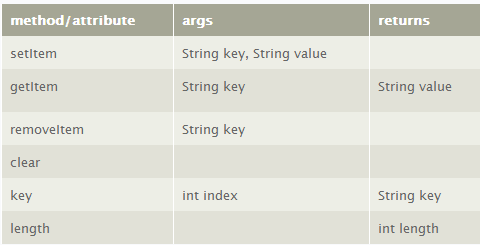
\includegraphics[width=0.9\linewidth]{graphics/chapter4/20}
\caption{Methods and attributes of local storage\cite{localstorageapi}}
\end{figure}


Here is an example of \textit{setItem} and \textit{getItem} in local storage.
\\

\begin{lstlisting}[language=html, caption= 
setItem example (Adapted from \cite{localstorageexample}),captionpos=b]
var foo = localStorage.getItem("bar");
// ...
localStorage.setItem("bar", foo);
\end{lstlisting}

In these application not a string but an array is stored inside the local storage. Here is an example how we put an empty array into a local storage.
\\

\begin{lstlisting}[language=html, caption= 
array into local storage,captionpos=b]
var names = [];
localStorage["favorites"] = JSON.stringify(names);
\end{lstlisting}
\
\

Here an example how we received the array form local storage.
\\
\begin{lstlisting}[language=html, caption= 
start timer function,captionpos=b]
var storedIds = JSON.parse(localStorage["favorites"]);
\end{lstlisting}

\newpage


\subsection{Slide Panel}
%%%%%%%%%%%%%%%%%%%%%%%%%%%%%%%%%%%%%%%%%%%%%%%%%%%%%%%%%%%%%%%%%%%%%
%link to slide panel chapter
%%%%%%%%%%%%%%%%%%%%%%%%%%%%%%%%%%%%%%%%%%%%%%%%%%%%%%%%%%%%%%%%%%%%%
In the upper left corner of the display exists a small button that calls the slide panel to open. More about slide panel in chapter 6.1.0.4)Slide Panel.
\\

\begin{figure}[h]
\centering
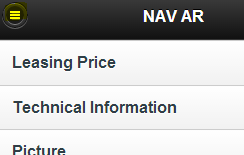
\includegraphics[width=0.5\linewidth]{graphics/chapter4/13}
\caption{Slide panel}
\end{figure}

After opening the slide panel more options are available. 
\\

\begin{figure}[h]
\centering
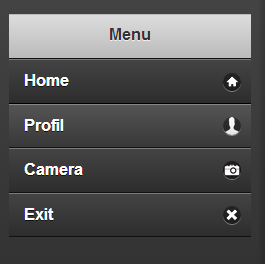
\includegraphics[width=0.5\linewidth]{graphics/chapter4/14}
\caption{Options of slide panel}
\end{figure}
\newpage

Here has the user four new options. He can return to the start menu with the display \textbf{home} or he can accesses his profile with \textbf{profil}. Also he can start to track a new car with \textbf{camera}. If the user doesn't want use the mobile application any more, he can close it the button \textbf{exit}. 
\\
\begin{lstlisting}[language=html, caption=Source code of slide panel options,captionpos=b]
<ul data-role="listview" data-theme="a">
  <li data-icon="home" >
    <a href="#" onclick="endtime();home();">
      Home
    </a>
  </li>
  <li data-icon="profil">
    <a href="profile.html" rel="external">
      Profil
    </a>
  </li>
  <li data-icon="camera" >
    <a href="#" onclick="endtime();trackClick();">
      Camera
    </a>
  </li>
  <li data-icon="delete">
    <a href="#" onclick="endtime();turnOff();">
      Exit
    </a>
  </li>
</ul>
\end{lstlisting}

The \textbf{home} button not only returns the user to the start menu but also ends the timer that has been started after a car was tracked. In addition, this timer is send straight to the NAV server.  
\\

Display \textbf{profil} calls to another display, in which the user can see his profile data. 
\textbf{Camera} function ends the timer and starts the tracking function. Exit ends the application.
\newpage


\subsection{Photo Gallery}
In this subchapter it describes the functionality of the photo gallery . The photo gallery is a feature of this project NAVAR. This feature shows the picture of the car which has been tracked by the NAVAR App. The Photo gallery is a plugin  from the photo swipe webpage. The Logic of the Photo swipe is implemented in a javaScript Library from photo swipe$\rightarrow$ klass.min.js. The functionality of the Design is defined in a css file$\rightarrow$ photoswipe.css. In this project it combined the Library form the photo swipe with the Library from jQuery Mobile. Furthermore the Table shows a Code snippet how to use the Library for this project:
\begin{figure}[h]
\centering
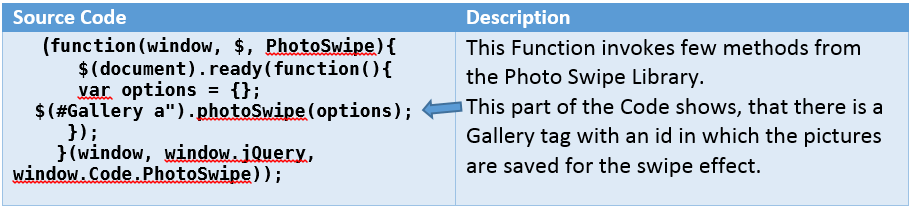
\includegraphics[width=1.0\linewidth]{graphics/photoswipe.PNG}
\caption{Photoswipe}
\end{figure}

Furthermore the pictures are saved on a server and in the Gallery we saved the URL of these pictures. The URL's are saved in an Array which has the id Gallery. For each car there is an Array with URL's of the pictures. Besides the photo swipe has the function to set a automatic Diashow.\\\\

\subsection{Sessionstorage}
Moreover the function called Sessionstorage is one of the big functionalities in this project. The Sessionstorage saves the value not persist, it means if the App is closed or has been ended  the value will be persistant . In the next Session or if the App has been started , there will be a new Sessionstorage. In this case the Project NAVAR uses the Sessionstorage to save the ID from the car, which has been tracked. Sessionstorage allows  to save a large amount of  key/value pairs and lots of text. This feature is impossible to do  via cookie. This kind of functionality uses  a protocol to save the Data. This protocol checks if the key and the value are a string, but if not it convert them to a string. Furthermore if a key was already present, its entry  has to be removed and the new one will be appended. The SessionStorage has it own methods for specific functionality.\\\\

First method is used to tell how many key/pair the SessionStorage contains. This method has the same function ,which tells the length of an Array, HTMLCollection \dots

\begin{figure}[h]
\centering
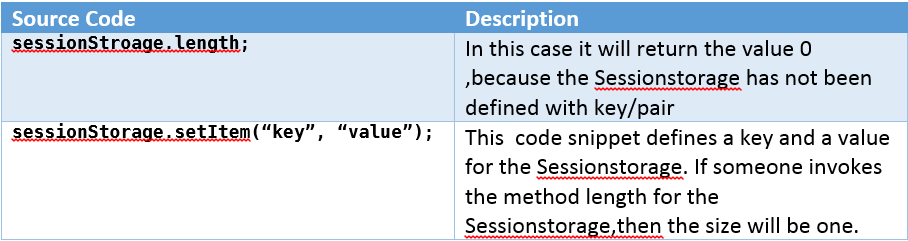
\includegraphics[width=1.0\linewidth]{graphics/sessionstorage1.PNG}
\caption{Sessionstorage}
\end{figure}

The second Method of Sessionstorage is called \textit{setItem(key:string,data:string)}.
 This method stores  a specified key  and the data. But if the key has been already stored and it uses the same key it will be overwritten. $\rightarrow$Example for setItem:\textbf{ sessionStorage.setItem('testkey','testvalue')}.
The third function is to get Data from the a specified key ,which has been already set. This method accepts any sort of string ,which has been used as key and returns the associated string as value or null if the key has not been stored before. Example:\\

\begin{figure}[h]
\centering
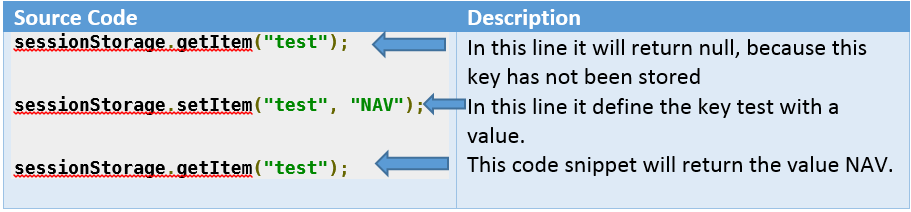
\includegraphics[width=1.0\linewidth]{graphics/sessionstorage2.PNG}
\caption{Sessionstorage}
\end{figure}

The last function is how to remove the key if it has no need for the Session. Example:
\begin{figure}[h]
\centering
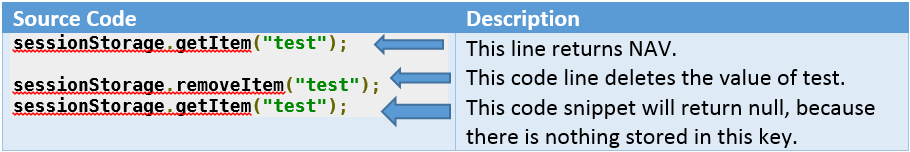
\includegraphics[width=1.0\linewidth]{graphics/sessionstorage3.PNG}
\caption{Sessionstorage}
\end{figure}

\subsection{Dynamic Selection of Colour}
This product has the feature to select the colour of the car . In the Technical Information the user has the opportunity to chose the colour of the Car, which has been tracked. The following code in the Figure shows how to create a dynamic selector with JavaScript:

\begin{figure}[h]
\centering
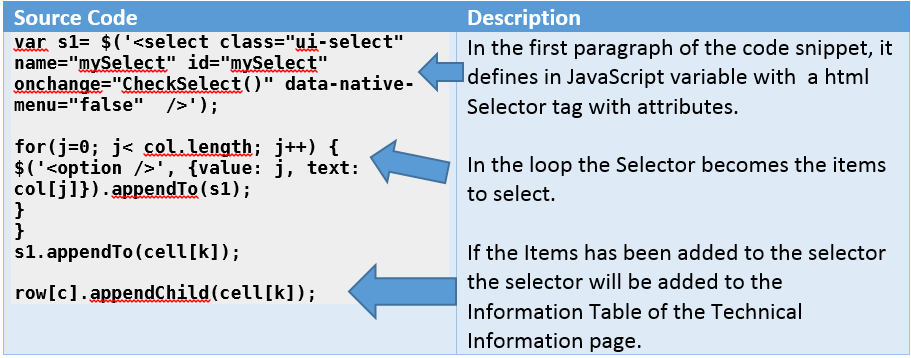
\includegraphics[width=1.0\linewidth]{graphics/Sessionstorage41.PNG}
\caption{Selector descritpion}
\end{figure}

\clearpage
The following picture shows how the Technical Info table looks like:

\begin{figure}[h]
\centering
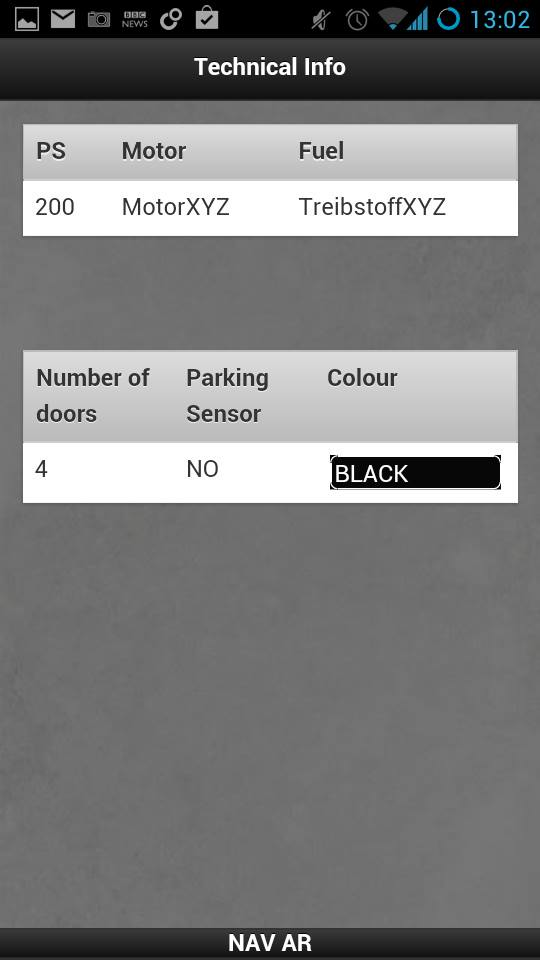
\includegraphics[width=0.4\linewidth]{graphics/chapter4/6.png}
\caption{Table}
\end{figure}
\clearpage
The second picture shows how the dynamic List of items from the Selector looks like:

\begin{figure}[h]
\centering
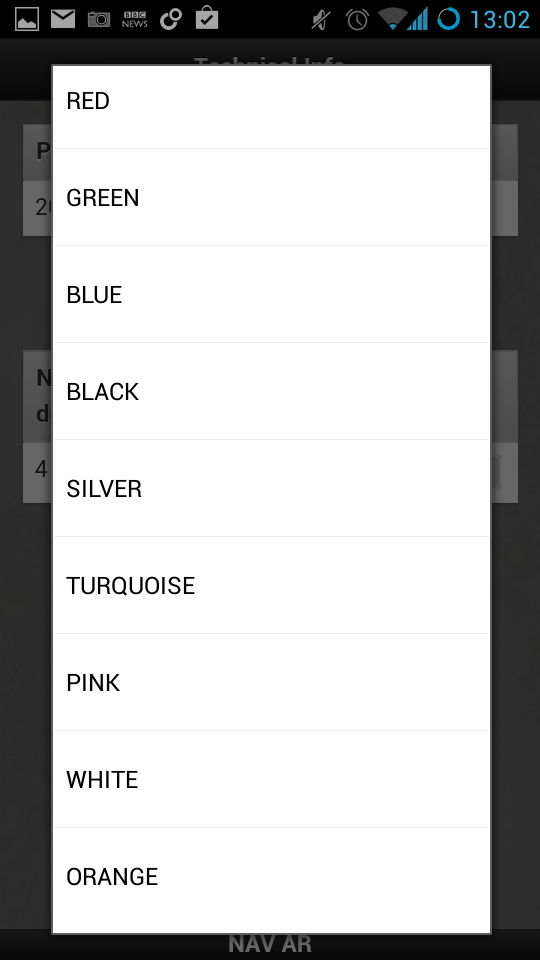
\includegraphics[width=0.4\linewidth]{graphics/chapter4/fg6.png}
\caption{Selector}
\end{figure}
\clearpage
Furthermore there is  a logic implemented which checks if the Colour is white or Black , that changes the colour of the font. The following code snippet shows how to write it:\\
\begin{figure}[h]
\centering
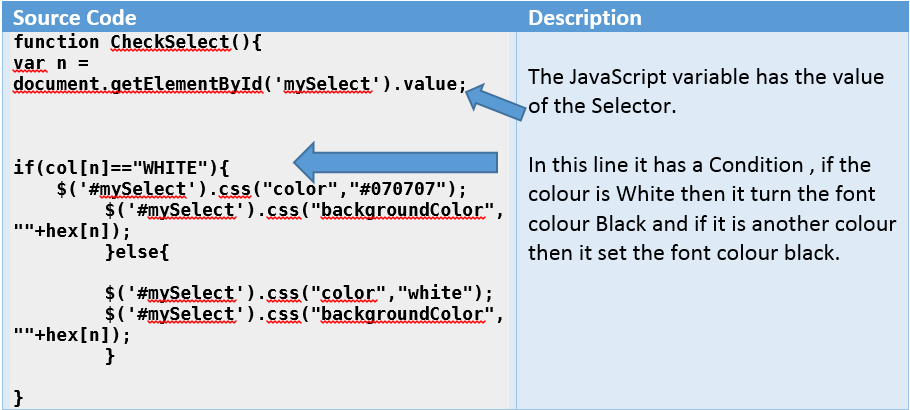
\includegraphics[width=1.0\linewidth]{graphics/bgfn.PNG}
\caption{Condition}
\end{figure}
%
% Chapter5

\chapter{Implementation in Android Java and Metaio Tracking} \label{chapter:metaio}
\section{Android Platform}
We choose Android because it is the most popular mobile platform and we already had experience in developing apps for android. 

\subsection{Android Operation System}
Android is an operating system based on Linux with a Java programming interface.
\\


Android is currently developed by Google.
\\


Android allows background processing, provides a rich user interface library, support
s 2-D and 3-D
graphics using the OpenGL libraries, access to the file system and provides an embedd
ed SQLite
database.\cite{androidDevTut}

\subsection{Android user interface components}
The most important user interface components ion android are: 

\begin{enumerate}
\item \textbf{Activity:} An Activity is the visible UI of an Android application. It contains so called \textit{widgets} for example buttons text-fields labels etc. to build a user interface. \cite{androidDevTut}

\item \textbf{Fragments:} Fragments
are components which run in the context of an
Activity. Fragments however make it easier to use build UIs for different sized devices.\cite{androidDevTut}


\item \textbf{Views and layout manager:} Views
are user interface widgets, e.g. buttons or text fields. They have attributes which can be used to configure their appearance
and behavior. (colour, size, onClick action, ..) \cite{androidDevTut}

\item \textbf{Layout XML:}
The user interface for Activities is typcally defined via XML files (layout files).\cite{androidDevTut}  But in this project we used HTML 5 and JQuery to make sure that the app could easily be ported to an other mobile platform just by re-writing the tracking logic to the specific system.

\item \textbf{Android Webview:} The WebView class is an extension of Android's View class that allows to display web pages as a part of the activity layout.\cite{androidWebView} As we already mentioned we choose this solution over plain Java-Android to achieve more platform independents.
\end{enumerate}   

\subsection{Develop an Android Application}
First of all the \textbf{Android SDK} is needed. The
Android Software Development Kit contains the necessary tools to create, compile and
package Android application.\cite{androidDevTut} 
\\


A compiled  
Android app is a \textbf{.APK} file which can be installed on a Android device. 
\\

The SDK also provides the \textbf{Android debug bridge}
(adb).A tool which allows to connect to an virtual or
real Android device.\cite{androidDevTut} We used this tool to test and debug our application.
 
\subsection{Android Manifest}
Every application must have an AndroidManifest.xml file in its root directory. The file describes essential information about the app. \cite{androidManifest}. For instance all activities, the app name, starting activity, size, etc. 
\\

It also contains al list of security permissions. We had to add the camera, internet, read\_owner\_data and get\_accounts permissions to implement all functions of our application. 


\begin{lstlisting}[language=xml, caption= 
extracts from our AndroidManifest,captionpos=b]
<uses-permission android:name=
	"android.permission.CAMERA" />
<uses-permission android:name=
	"android.permission.INTERNET" />
 <uses-permission android:name=
 	"android.permission.READ_OWNER_DATA" />
<uses-permission android:name=
	"android.permission.GET_ACCOUNTS" /> 
...
<!-- define an activity -->
<activity
	android:name=".TrackLogic"          
</activity>
\end{lstlisting}

\subsection{Creating an activity}
Every Android activity has to extend the \textbf{Activity} class and override the \textbf{onCreate} Method. onCreate gets executed when the activity is initialized.

\subsection{Android web-view}
We used the Activity sub-class \textbf{DroidGap} from \textbf{phonegap} to build activities. With this class it is easy to load webpages as view. 
\\



\begin{lstlisting}[language=java, caption= 
extracts from our source code,captionpos=b]
public class MainMenue extends DroidGap {
	...
	public void onCreate(Bundle savedInstanceState)
	{
		..
		super.loadUrl(
		"file:///android_asset/file.html", 10);
		...
	}
}
\end{lstlisting}

The method \textbf{loadUrl} loads any web-page, doesn't matter if the URL is internal or external. It is also possible to pass an additional int time out parameter.   


\subsection{Java JavaScript Communication}
In the section above we mentioned that we used html pages to create the view of our application. Because of that we had to find a way to pass variables through, the in Java written activity, to the web-view. We accomplished that by using JavaScript. Again the activity has to extend the \textbf{DriodGap} class.
\\



First javascript must be enabled:
\begin{lstlisting}[language=java,captionpos=b, caption=??????]
super.appView.getSettings().setJavaScriptEnabled(true);
\end{lstlisting}

Now its possible to pass variables to the html view:
\begin{lstlisting}[language=java]
int a=1;
super.loadUrl("javascript:{var myVariable=\""+a+"\";}");
\end{lstlisting}


\subsubsection{JavaScript Android Interface}
With such an interface it is possible to call activity methods form JavaScript. We needed them to react on button clicks from inside of the html view.  
\\

First we had to write a JavaScript function:
\begin{lstlisting}[language=html, captionpos=b]
<script language="Javascript">
function trackClick() {
        MyTracking.performClick();
    }
</script>
..
<!-- set onCLick Action -->
<a href="#" onclick="trackClick();">Camera</a>
\end{lstlisting}





Then add a JavaScript interface to the activity:
\begin{lstlisting}[language=java, caption=?????, captionpos=b]
super.addJavascriptInterface(new Object()
{
	public void performClick()
	{
		//react to button click
	}
},"MyTracking");
\end{lstlisting}

\section{Working with the Metaio SDK}
We used the Metaio SDK track and identify 3D or 2D Objects.


\subsection{Who is Metaio}
\begin{quotation}
"Metaio is the worldwide leader in Augmented Reality research and technology. Serving over 80,000 developers with over 1,000 apps for enterprise, marketing, retail, publishing and industrial cases,
 
 
Metaio's AR software reaches over 30 Million consumers across the world." 
\begin{flushright}
(Metaio GmbH)
\end{flushright}
\end{quotation}

\subsection{Other Augmented Reality SDK's}
There are many other augmented reality technologies on the market: 
\begin{enumerate}
\item \textbf{Qualcomm Vuforia}: The Vuforia platform is mostly used for image recognition.

\item \textbf{Total Immersion D'Fusion}:
D'Fusion is the world's most widely-used commercial Augmented Reality solution. Unfortunately there are no free versions.

\item \textbf{Wikitude}: Wikitude is a powerful augmented reality sdk.However the cheapest SDK version costs 99\$.

\item \textbf{String}: String only recognises framed images. So this SDK was unusable for our application.  
\end{enumerate} \cite{augmentedRealitySDk}

In the End we choose Metaio SDK not only because our client recommended it but also because Metaio is a very powerful SDK. Unlike like most other technologies it has a free version and can track 3D objects. 
\\



Metaio also has a very big user community with a help-desk and many tutorials.   
 
\subsection{Metaio Toolbox}
The metaio Toolbox is an application used to create or edit 3D tracking maps of all textured objects in your surrounding.The created Maps than can be used in the Metaio SDK. We used the Toolbox-App to create 3D Maps of the cars our application is tracking.
\\ 

The Toolbox also allows you to play or edit AREL scenes. The AREL scene created in the metaio Creator can be directly played in the Toolbox. The geometries transformations can be edited in the Toolbox.
\\


Furthermore, the Toolbox also has camera calibration function that allows you to determine camera parameters of your device.  The Metaio Toolbox is a simple APP which is a available for Android and IOS. The APP can simply be downloaded and installed from Apple App-Store or Google Play.\cite{metaioToolBox}

Process of creating a Map:
\begin{enumerate}
\item Download and install Metaio Toolbox.
\item Open The App.
\item Tab on \textit{3D} Maps and than on \textit{new Map}. (It is also possible to edit existing map)
\item After that the camera opens and a Object can be tracked.
\end{enumerate}    
\begin{figure}[htbp]
\centering
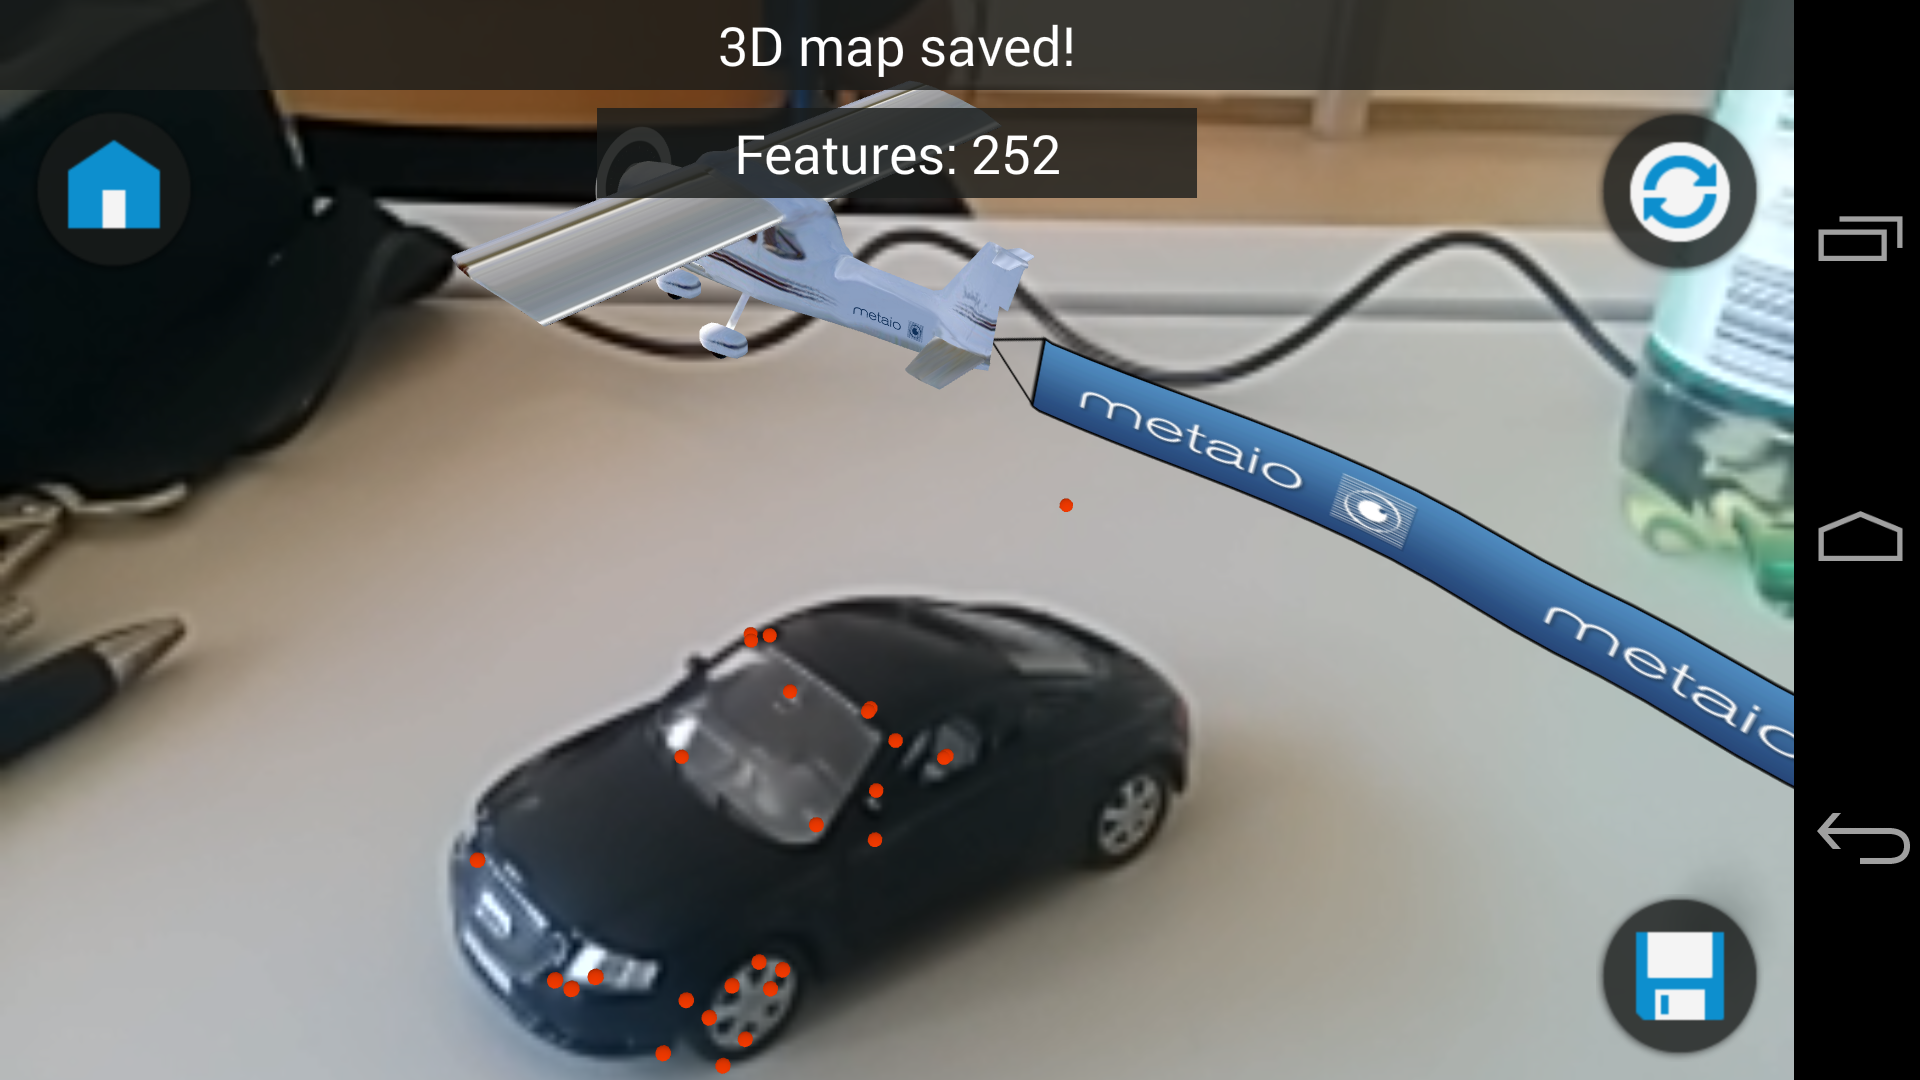
\includegraphics[width=\textwidth,height=\textheight,keepaspectratio]{graphics/tracking.png}
\caption{Metaio Tool Box}
\end{figure}
The red dots in the figure show the tracking points, the \textit{FEATURES} count shows how many tracking points have been placed. The more points the better can the object later be tracked by an application.

\subsection{AREL ( Augmented Reality Experience Language )} 
AREL ( Augmented Reality Experience Language ) is a JavaScript binding of the metaio SDK's API in combination with a static XML content definition

With Areal Scenes its possible to create a script with all tracking object and their behaviour, that scene than can be run by any metaio SDK. That's how you are able to create one platform independent Augmented Reality experience with AREL instead of using platform specific programming languages.
\begin{figure}[htbp]
\centering
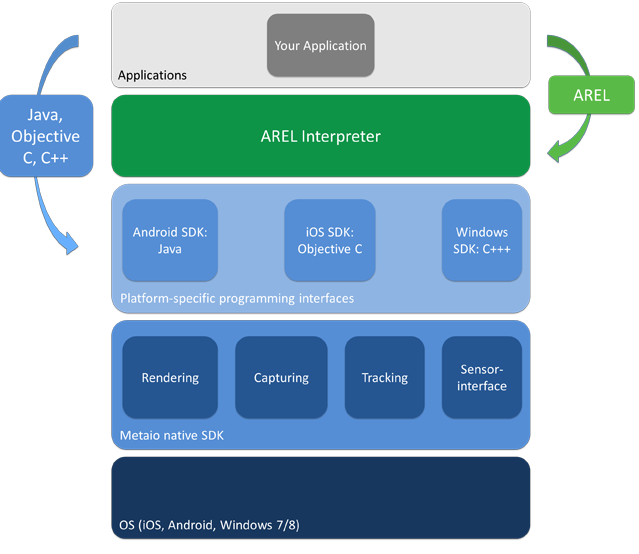
\includegraphics[width=\textwidth,height=\textheight,keepaspectratio]{graphics/arel.PNG}
\caption{AREL}
\end{figure}

AREL consists of the following parts:
\\

A XML Part which defines the content that should be loaded (3D-Models,Maps) and their size, position, transformation, etc. 
\\





The HTML 5 layer, this part provides graphical user interface and interacts using the JavaScript bridge with the metaio SDK. The AREL JavaScript bridge is a javascript library that allows to communicate with the Metaio SDK. All callbacks from the SDK are forwarded to the JavaScript Logic. \cite{metaioToolBox} 
\\

However AREL scenes where not use in the project because they only offered a limited size of Actions. For instance we needed to get the ID of the tracked object to determine which car had been recognized. It turned out that this is a much more difficult process in AREL so we wrote the whole logic in Java using the Metaio SDK.     

\subsection{Tracking XML}
The Tracking XML file is an XML file which can be created by the Metaio Creater or written by hand. It contains all of the tracking data. (3D Maps, etc. ..)
\begin{lstlisting}[language=xml, caption=Tracking XML example,captionpos=b]
<?xml version='1.0' encoding='UTF-8'?>
<TrackingData>
	<Sensors>
	<Sensor subtype='ML3D' type=
		'FeatureBasedSensorSource'>
		<SensorID>TrackingObject 1</SensorID>
		<Parameters>
		<featureorientationassignment>regular
		</featureorientationassignment>
		</Parameters>
		<SensorCOS>
		<SensorCosID>
		08921d8412c4de43d04eefc13c28ee3b
		</SensorCosID>
		parameters>
		 <numextensiblefeatures>
		 	0
		 </numextensiblefeatures>
		 <mintriangulationangle>
		 	6
		 </mintriangulationangle>
		 <map>
		 08921d8412c4de43d04eefc13c28ee3b.f3b
		 </map>
		 <MinMatches>15</MinMatches>
		 <DesiredMatchesRatioExtensible>0.35
		 </DesiredMatchesRatioExtensible>
		 <NumExtensibleFeatures>250
		 </NumExtensibleFeatures>
		</parameters>
		</SensorCOS>	
	</Sensors>
</TrackingData>
\end{lstlisting}
All tracking Objects have to be added into the \textbf{Sensors} element. Every new object needs a \textbf{SensorCosID}, the name of the object. The \textbf{<Parameters>} element describes the 3D Map for the object. The map has to be in the same folder like the tracking xml. Other parameters are for instance the  \textbf{<MinMathes>} element, it describes how many points have to match so that the object gets recognised. Metaio has not really got a documentation for the Tracking XML therefore we choose to let the Metaio Creator create the xml file.


\subsection{Extracting the Tracking XML in Android}
In order to use xml file with the Metaio SDK, the tracking xml has to be placed in the \textbf{assets} folder of the android project.
\\


The files than have to be extracted by the \textit{AssetsManager} to make them accessible to the metaio SDK. This has to bee done in an Android \textit{AsyncTask}.
\\

The AsyncTask enables proper and easy use of the UI thread. This class allows to perform background operations and publish results on the UI thread. AsyncTasks should ideally be used for short operations (a few seconds at the most.) For threads that need to be running for long periods of time, it is recommended you use the various APIs provided by the java.util.concurrent pacakge such as \textit{Executor}, \textit{ThreadPoolExecutor} and \textit{FutureTask}.\cite{andoirdAsyncTask} 

\begin{lstlisting}[language=java, caption=Extracting Assets,captionpos=b]
private class AssetsExtracter extends AsyncTask
{		
	@Override
	protected Boolean doInBackground(.. 
	{
		try 
		{
			// Extract all assets
			AssetsManager.
				extractAllAssets(...);
		} 
		catch (IOException e) 
		{
			//Error Messages
		}
			
		return true;
	}
		
	Override
	protected void onPostExecute(Boolean result) 
	{
		// Asset Path to the Tracking xml
		final String arelConfigFilePath = 
		  AssetsManager.
		  getAssetPath("Tracking.xml");
		//Starting new Activity  
		Intent intent = 
		new Intent(getApplicationContext(), 
		 TrackLogic.class);
		intent.
		putExtra(getPackageName()+".AREL_SCENE", 
		  arelConfigFilePath);
		startActivity(intent);

		finish();
	  }
}
\end{lstlisting}
The AsyncTask gets executed like this:

\begin{lstlisting}[language=java, caption=executing AsyncTask,captionpos=b]
 AssetsExtracter asyncTask=new AssetsExtracter();
 //executing the task
 asyncTask.execute(0);
\end{lstlisting}





Android first runs the \textit{doInBackground} method, in this case the method extract all Assets using the Metaio 	AssetsManager: 	\textit{AssetsManager.extractAllAssets(...);}. After this method ends successfully the \textit{onPostExecute} method gets called.
\\


onPostExecute extracts the path to the tracking.xml and than starts the TrackingLogic class. This Activity is where the tracking happens.

\subsubsection{Loading the Tracking XML}
The TrackingLogic class in our project loads the tracking xml using the Metaio SDK:
\begin{lstlisting}[language=java, caption=executing AsyncTask,captionpos=b]
String filepath = 
AssetsManager.getAssetPath("Tracking.xml");
...
// set the tracking configuration
 metaioSDK.setTrackingConfiguration(filepath); 
\end{lstlisting}

\section{Track Objects}
In order to run the camera and start the tracking process we wrote a new Activity which has to extend the Metaio \textbf{ARViewActivity}. Important methods provided by this class:
\begin{enumerate}
\item \textbf{loadContents():}This Method load the tracking xml.
\item \textbf{onTouch(View v, MotionEvent event):} By overwriting this method you can set what happens when the user touches the screen. 

\item \textbf{onGeometryTouched(final IGeometry geometry):} Metaio provides the possibility to draw 3D and 2D Models on the screen while tracking with the camera on, the method determines what happens when this geometry gets touched 

\item \textbf{onTrackingEvent(TrackingValuesVector trackingValues):} 
\\
One of the most important methods.onTrackingEvent describes what happens when an object gets tracked successfully. We overwrote this method to get the ID of the tracked Object. After the object hast been tracked the Main Menue activity with all specific car informations gets started.   
\end{enumerate} 
\begin{lstlisting}[language=java, caption=Tracking Event,captionpos=b]
public void onTrackingEvent(TrackingValuesVector tV)
{
 //Check through all maps 
 for (int i=0; i<tV.size(); i++)
 {
  final TrackingValues v = tV.get(i);
  if (v.isTrackingState())
  {
	Intent inte=
	new Intent(getApplicationContext(),Menue.class);
	//get id of tracked object
	inte.putExtra("id",""+v.getCoordinateSystemID());
	startActivity(inte);
	//close activity
	finish();
  }
				
 }
}
\end{lstlisting}
\section{Get Email Account from an Android device}
This product has  a small feature, it saves the email address from the smartphone and this email Address will be sent to the Navision Server. In this paragraph it describes how the project team implemented the feature in this Application.
Description \& Codesnippet:
This method will be invoked by the method getmail. This method will be explained in the next row. The getAccount() method  filters the Google Accounts . This happened through the Method getAccountsByType('com.google');.
Furthermore if the first object of the Account Array is bigger then the value of Account  it will be returned.

\begin{lstlisting}[language=java, caption= Accounts,captionpos=b]
private static Account 
	getAccount(AccountManager accountManager) {
Account[] accounts = 
	accountManager.getAccountsByType("com.google");
Account account;
if (accounts.length > 0) {
	account = accounts[0];     
} else {
      account = null;
}
   return account;
}

\end{lstlisting}

In this  Method it returns the Account object as String value. This happens through the Accountmanager and this method invokes the getAccount method. With the account Object it checks if it null if not then it returns the email address as String object.


\begin{lstlisting}[language=java, caption= Email,captionpos=b]
static String getEmail(Context context) {
AccountManager accountManager = 
AccountManager.get(context); 
Account account = getAccount(accountManager);
if (account == null) {
	return null;
} else {
    return account.name;
	}
}
\end{lstlisting}
The Email Address will be saved in a file , so the application  have to read the email address from the file. %


\chapter{Design Concept} \label{chapter:desgin}

\section{Design concept with JQuery Mobile Framework}
In this chapter it will be explained how the project NAVAR used the jQuery Mobile Framework,CSS3 and HTML5 to create the user Interface of the APP NAVAR. This chapter will describe how to use  the components of the JQuery mobile framework. The reason why the project NAVAR uses Javascript,HTML5,
CSS3 and jQuery Mobile for the user interface is, that the design can be used for other platforms. This pictures shows how the app is built:
\\\\
\begin{figure}[htbp]
\centering
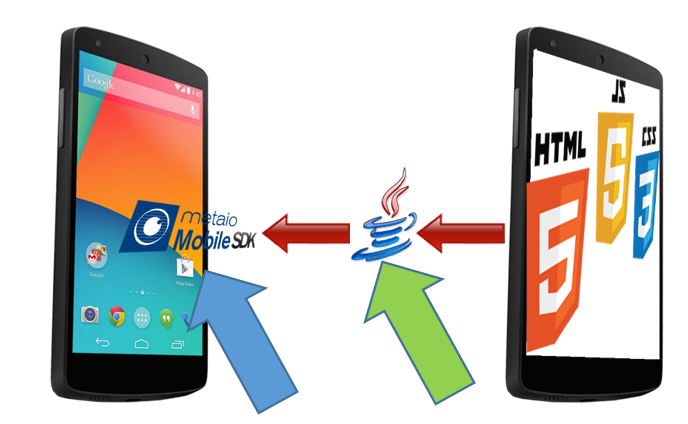
\includegraphics[width=240pt,height=180pt,keepaspectratio]{graphics/AppStructure.PNG}
\end{figure}
\\\\
The blue arrow shows the SDK of Metaio. The Metaio SDK will be explained in the chapter Implementation. Moreover, if Metaio GmbH creates a SDK for another platform, so it should be necessary to change the SDK and Java Components of this project NAVAR(green arrow). NAVAR was built with modularity. There is then no need to change something in the user interface because it can be used for every mobile platform.
\\\\

\subsubsection{jQuery Mobile Page}
The Basic of jQuery Mobile is to create a blank page and then to define the components such as Button or Listview, etc, which defines the interaction for the user interface.  The blank page is a HTML File. It has the same basic html tag structure. The main benefit of the jQuery Mobile Framework is, there are attributes for each component or HTML tag such as:
\\
\begin{itemize}
\item data-theme $\rightarrow$ to Define the colour of a component
\item data-role $\rightarrow$ defines the components in HTML such as Button,Listview or Link
\item data-icon $\rightarrow$  defines which icon should be used for the HTML component.
\end{itemize}

There are more data- attributes which are defined in this jQuery Mobile API:  http://demos.jquerymobile.com/1.2.0/docs/api/data-attributes.html\\\\     
\newpage The following Codesnippet will show  the Source Code looks for a jQuery Mobile page:

\begin{lstlisting}[language=html,caption= jQuery Page,captionpos=b]
<html>
<head>
    <title>NAV-AR</title>
    <link href="css/jquery.mobile-1.3.2.min.css" 
    rel="stylesheet" type="text/css"/>
    <script src="js/jquery-1.9.1.min.js" 
    type="text/javascript">
    </script>
    <script src="js/jquery.mobile-1.3.2.min.js" 
    type="text/javascript">
    </script>
    <script type="text/javascript" src="js/notifier.js">
    </script>    
<body>
<div data-role="header">
</div>
<div data-theme="a" data-role="footer" 
data-position="fixed" data-id="footer">
    <a class="ui-btn-left" href="index.html" 
    rel="external">Back</a>
</div>
</body>
</html>

\end{lstlisting}

Listing 2.1 shows how to add the Library into a HTML and how to create Header, Footer from jQuery Mobile Framework. Furthermore how to use the data-role Attribute, it is often defined in HTML container Tag called div.\\\\

\subsubsection{Mainmenu}
In this segment it will be explained how to use the Listview to create a Menu with navigation form. The usage of Lists are for data display, navigation, result lists, and data entry. First of all ,to create a  Listview, the html file have to include jQuery Mobile library$\rightarrow$Code:
\begin{lstlisting}[language=html,caption= Input Library,captionpos=b]
<script src="js/jquery.mobile-1.3.2.min.js"
 type="text/javascript"></script>

\end{lstlisting}

It is possible to create a dynamical Listview, but for the dynamic function it needs JavaScript. For the menu of the APP the list view is static. This Figure shows the syntax for the Listview:

\begin{figure}[htbp]
\centering
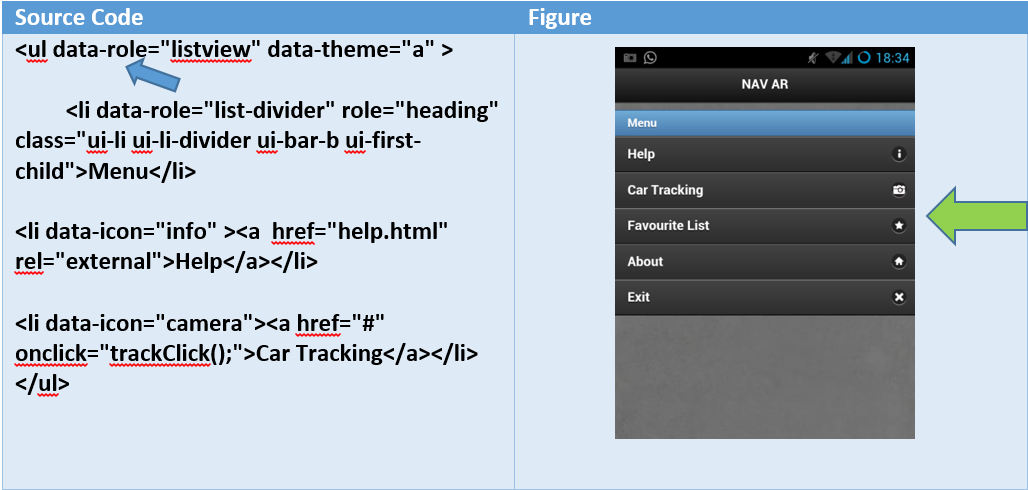
\includegraphics[width=1.0\linewidth]{graphics/Menu.PNG}
\caption{Menu Page}
\end{figure}

Jquery Mobile uses the HTMLTags  to create a component of  jQuery mobile and to define the data-role. Data-role is an attribute which can be used if the JQuery Mobile Library is included(Blue arrow). For this project the List items(Green Arrow) are linked to another html Files or it invokes a Function.\\\\

\subsubsection{Slide Panel}
The Slide Panel is one of the big functionalities of the jQuery Mobile Framework. With the Slide Panel it is possible to make it easy to create menus, collapsible columns, drawers, inspectors panes and more. The Panel have to be defined in a jQuery Mobile Page. Furthermore the Panel can not be placed outside of the page. The Figure shows ,how the panel looks like with the code snippet of this project NAVAR. The main point is to a create panel and to define the attribute data-role to a panel(Blue arrow.)\\\\
Afterwards the project has List Items in the panel for a menu. The user can navigate easily through the user interface with this feature.\cite{Panel}


\begin{figure}[h]
\centering
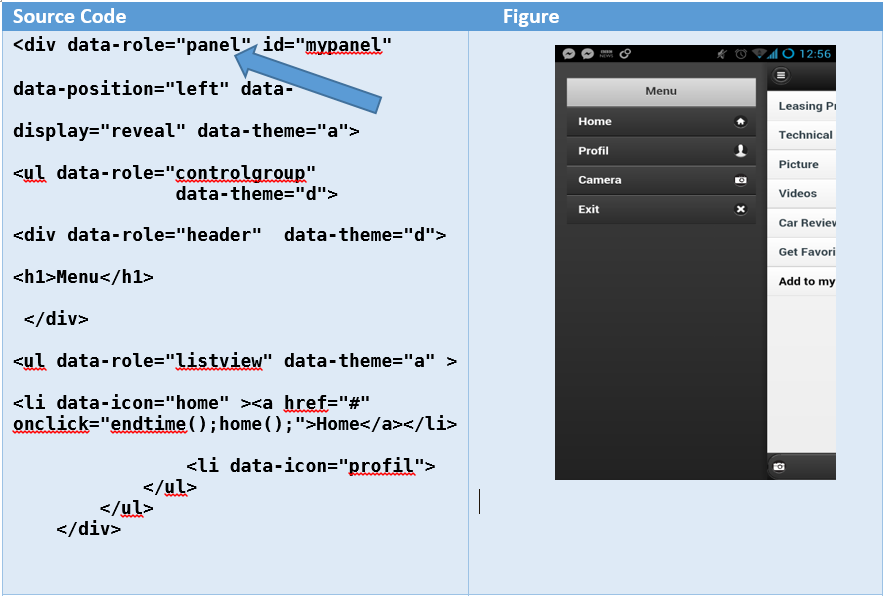
\includegraphics[width=1.0\linewidth]{graphics/SPanel.PNG}
\caption{Slide Panel}
\end{figure}
\clearpage

The Panel has to defined in the header of jQuery Mobile page or as Button function. This  code snippet  shows how to do it. First all the Panel has to been defined with a id to get reference of it.
Codesnippet:
\begin{lstlisting}[language=html,caption= Panel definition in Header,captionpos=b]
<div data-role="header">
        <h1>NAV AR</h1>

         <a href="#mypanel" data- 
          icon="bars" data- 
        iconpos="notext">Menu</a>

    </div>
s
\end{lstlisting}
\subsubsection{jQuery Mobile Table}
JQuery Mobile Framework has the feature to create a table. In this project tables are very important, because the Information from the Navision Server will be list in a table. The following code snippet will show how it works :
\begin{figure}[H]
\centering
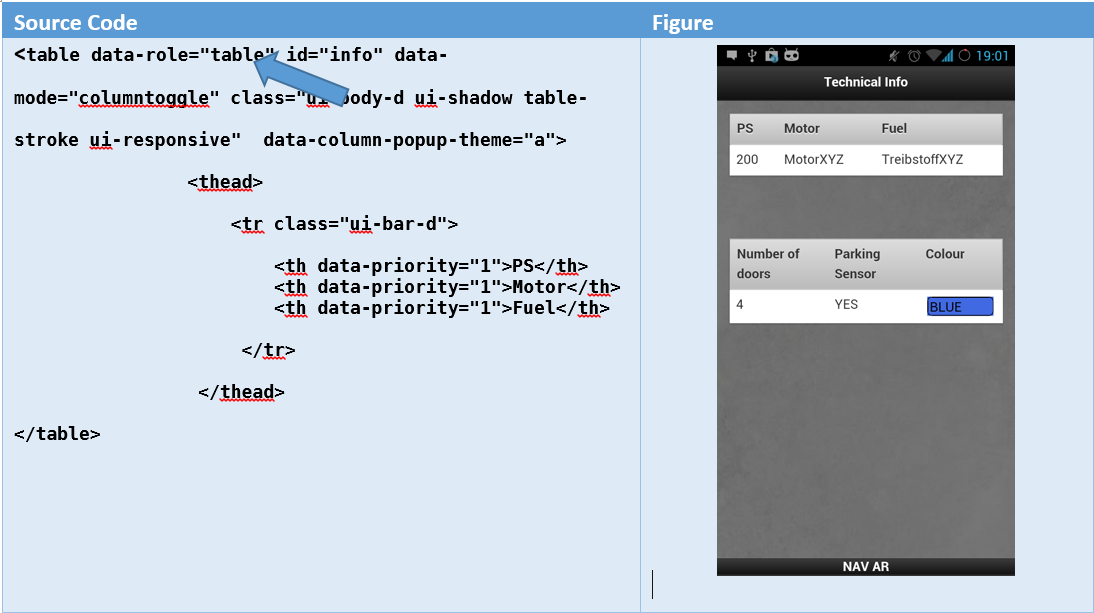
\includegraphics[width=1.0\linewidth]{graphics/Table.PNG}
\caption{Table}
\end{figure}
shows the attribute data-role should have bee defined as 'table'(Blue Arrow).With the other attributes such as:
Data--mode, data--column--popup--theme. With these attributes it is possible to define the appearance of the table.

\newpage
\section{Video Gallery}
The video Gallery in our mobile-application gives the user the possibility to watch test reviews and commercial videos of the tracked car.
\\

   
For implementing the YouTube car video gallery we used \textbf{jquery} and the jquery plug-in \textbf{jquery.youtubevideogallery}. The Design and CSS files were taken from Jack Moore's plug-ins. \cite{jqueryVideo}. His great work makes it possible to dynamically scale the size and position of the video-boxes so that they perfectly fit on every device screen! 
\\

As one can see in the figure on the next page the position and size automatically adjust to the 3 different screen sizes.    

\begin{figure}[H]
\centering
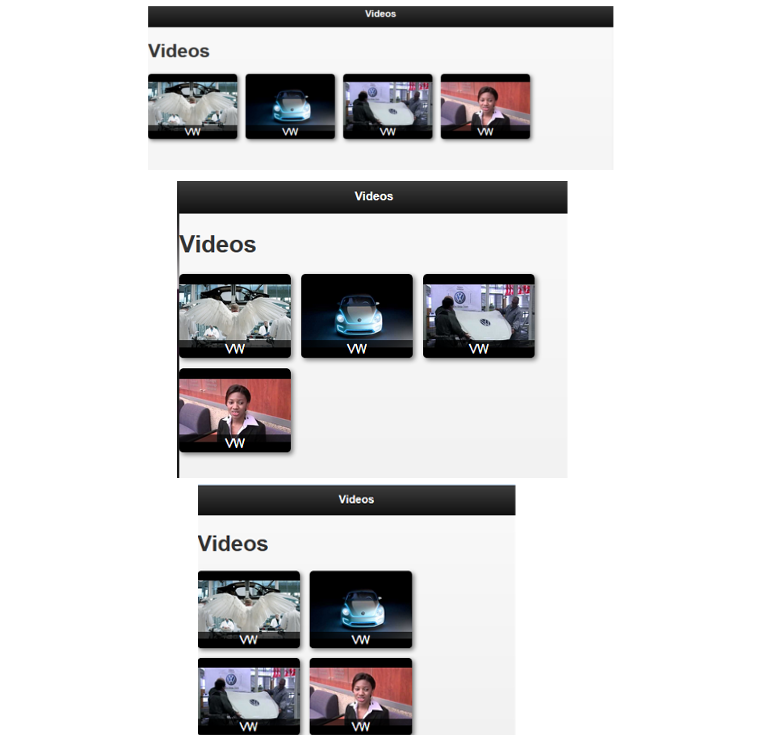
\includegraphics[width=\textwidth,height=\textheight,keepaspectratio]{graphics/dynamic.png}
\caption{dynamically fit to device screen}
\end{figure}  

\newpage
\subsection{Implementation}
We wrote a JavaScript script that appends an array of different YoutTube video url to an \textbf{ul} tag which uses the \textbf{youtube-videogallery} class.   
\begin{lstlisting}[language=html, caption= 
extracts from the video gallery src,captionpos=b]
<ul id="Gallery" class="youtube-videogallery">
	<script>
	... 
	//append video urls
	for (var i=0; i<videos.length; i++){
		$("#Gallery").append(videos[i]);
	}
	</script>
</ul>
<!-- Use jack Mores .js for the gallery -->
<script>
    $(document).ready(function(){
        $("ul.youtube-videogallery").
        youtubeVideoGallery( 
        {plugin:'colorbox',assetFolder:'../'} );
    });
</script> 
\end{lstlisting}
%
% Chapter7
\chapter{Streaming} \label{chapter:Streaming}
This chapter explains the network structure of the whole project and how the connections between the servers and the app are done.
\subsection{General network}
The following figure shows the detailed network set-up and application flow of the project.
\begin{figure}[htbp]
\centering
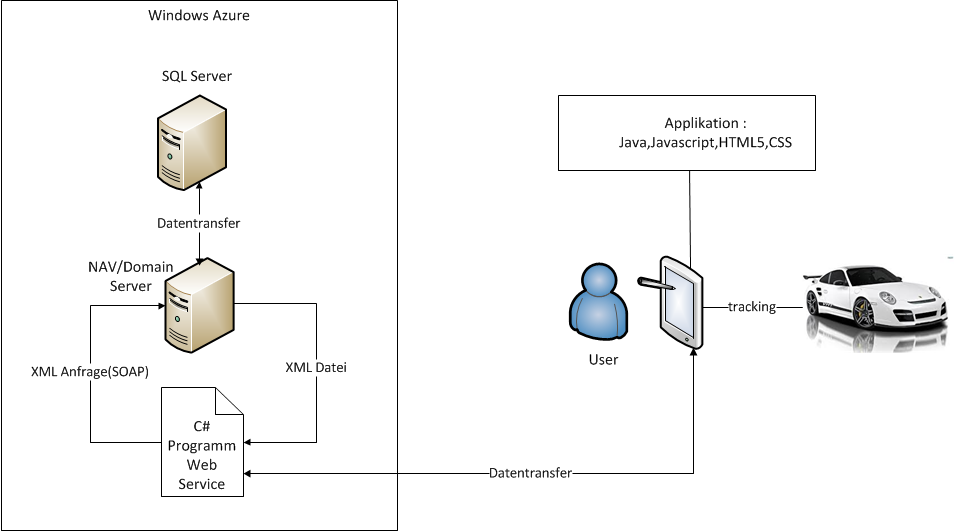
\includegraphics[width=\textwidth,height=\textheight,keepaspectratio]
{graphics/networkoverview.png}
\caption{network overview}
\end{figure}

The front end consists of an application which runs on a mobile device and is operated by a user. On the back end is a Microsoft Windows Azure platform which contains the following two server instances. The server with Microsoft SQL in the top of the graphic is for saving and processing the data. The bottom server in the graphic, the main server on which runs Microsoft Navision 2013(NAV) and a domain for communicating with the SQL server. Both of these server operation systems are windows server 2008 R2. The C\# application is installed as a windows service and is used to communicate between back end and front end.

\subsection{C\# Application}
The application consists of two important main parts. The first part is the communication between the Navision server and the C\# program. To solve this problem it uses a Navision web service to access and receive the needed data. The Navision web service will be explained in the following sub chapter ''Navision Server''. When the set up of the NAV web service is done it can be simply added as a web reference in Visual Studio to access it in the code.
\\\\
\begin{description}
   \item[The application has three web references]~\par
   \begin{enumerate}
      \item NavArCarData, which is used to get all information about a tracked car. 
      \item NavArTrackingHistory , which is used to save a history of tracked cars.
      \item	NavArUserData, which is used to save data from the user. 
   \end{enumerate}
\end{description}

\begin{figure}[htbp]
\centering
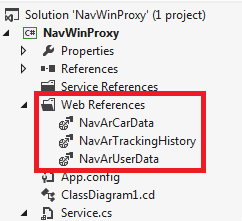
\includegraphics[width=40mm,height=\textheight,keepaspectratio]{graphics/webref.png}
\caption{web reference}
\end{figure}
The web references can be accessed via the code in Visual Studio.
\newpage
\definecolor{bluekeywords}{rgb}{0.13,0.13,1}
\definecolor{greencomments}{rgb}{0,0.5,0}
\definecolor{redstrings}{rgb}{0.9,0,0}
\lstset{language=[Sharp]C,
  breaklines=true,
  commentstyle=\color{greencomments},
  keywordstyle=\color{bluekeywords},
  stringstyle=\color{redstrings}
}
\subsubsection{Read from the web service}
\begin{lstlisting}[caption=Example reading webservice]
//use the created web reference
using NavWinProxy.NavArCarData;
//Create a service object
NavArCarDataPage_Service service = new NavArCarDataPage_Service();
//set user credentials which have access rights to the Navision server
service.Credentials = System.Net.CredentialCache.DefaultCredentials;
//create a new Object for storing the data
NavArCarDataPage carData = new NavArCarDataPage();                
//read the data which a specific id
carData = service.Read('1');
//check if the id exists
if (carData != null){
   //access data and store data
   string accessData=carData.Feld1;
}
\end{lstlisting}      

In this code example the web reference can simply accessed with the using statement and a service object. After that the credentials are set with ''System.Net.CredentialCache.DefaultCredentials''.
These are the default credentials from the user who runs the program. After that a  NavArCarDataPage object is created for storing data from the web service. Then the data can easily read with service object with service.Read(String ID)  method.
\newpage
\subsubsection{Write to the web service}
\begin{lstlisting}[caption=Example writing to web service]
 public string insertProfileData(string androidEmail,string profileEmail, string firstName, string lastName, string hash)
        {
        //create the service object
        NavArUserDataPage_Service service = new NavArUserDataPage_Service();
        //set user credentials which have access rights to the Navision server
        service.Credentials = System.Net.CredentialCache.DefaultCredentials;
        //read the user data from a specific google mail address
        NavArUserDataPage userData = service.Read(androidEmail);
        //check if the email exis 
        if (userData != null)
            {
            //set the profile data
            userData.Feld2 = profileEmail;
            userData.Feld3 = firstName;
            userData.Feld4 = lastName;
            //update the navision database with the new data
            service.Update(ref userData);
            }
            else return "fail";
                return "success";
            }
            else return "fail";
        }
\end{lstlisting}
The beginning of the example code is similar to reading from the web service.At line number 8 profile data are read with a google email adress and is checked if it exist. If it exist the attributes for are profile email,first name and last name is set and it get updated with .Update(Object to Update) method.The shown example method is simply used for inserting/updating profile data from the application in the Navsion Server 
  
\newpage
\subsubsection{Provide a web service}

The other important part of this application is to provide a web service for communication with the mobile devices.  To provide the functionality the C\# program uses ''System.Service.Model.web'' which contains several methods for implementing a web service.  In the following code example an operation contract is made to publish specific methods so that the mobile devices can access these methods.
\\\\
\begin{lstlisting}
[ServiceContract]
    public interface IOrderService
    {
        [OperationContract]
        [WebGet(UriTemplate = "getKFZInfo/{id}/{hash}",ResponseFormat =           
        WebMessageFormat.Json,RequestFormat = WebMessageFormat.Json)]
        string getKFZInfo(string id,string hash);
    }
\end{lstlisting}

This example consist of one method ''getKFZInfo'' with two parameters id and hash. It returns the car information with the given id if the hash is correct. The hash value is used to prevent access from other unwanted programs. The method could be access via the web url ''serveradress/getKFZInfo/id/hashvalue''. An invocation with the web browser would look like this:  127.0.0.1/getKFZInfo/5/ac3rf229f1fb88a8719e5f6d29443545
\newpage
\subsubsection{Communication from mobile device to the C\# App}

The mobile app access the web service of the C\# application within JavaScript. Ajax is used for providing the communication between the user and the server. In the following code example an Ajax request to the server is shown.


\begin{lstlisting}[language=html, caption=readcarname example]
function readcarname(cname){
        $(document).ready(function () {
            $.ajax({
                type: "GET",
                url: "http://tgm.cloudapp.net:9090/rest/getKFZInfo/"
                +cname+"/ac73f229f1fb88a8719e5f6d295bee45?callback=?"
                ,async: false,
                dataType: 'JSONP',
                success: function(data){
                    globalcarname= data.split(';')[0];
                }
            });
        });
    }
\end{lstlisting}
This example consist of one function readcarname(cname) which sends an Ajax request with a given parameter to the server. The first part of the url in the request represents the azure domain: http://tgm.cloudapp.net:9090 where the C\# application is hosted and the second part is the method which should be called. The dataType is JSONP so that it is possible to transfer and receive data over different domains. The success method in the Ajax request will be triggered after the server sends the data back. In this example the response data from the server is stored in the variable ''globalcarname''.
\newpage
\subsection{Navision Server}
For storing and receiving the important data for the mobile application a Navision Server 2013 is used.
\subsubsection{Table structure}
\begin{description}
   \item[The table structure contains three tables for storing]~\par
   \begin{enumerate}
      \item NavArTrackingHistory 
      \item NavArCarData
      \item	NavArUserData. 
   \end{enumerate}
\end{description}

The NavArTrackingHistory table is used to save the tracking history of a user to the database. It has six columns for saving the tracking history of a user.
\newline
\begin{figure}[htbp]
\centering
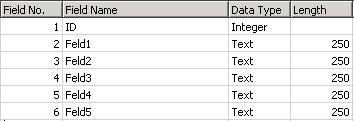
\includegraphics[width=100mm,height=\textheight,keepaspectratio]{graphics/trackingtable.png}
\caption{NavArTtrackingHistory table}
\end{figure}
\newline
  The following figure shows an example entry. This entry consist of a unique ID, email address, ID of the tracked car, start time, end time and duration.  
\begin{figure}[htbp]
\centering
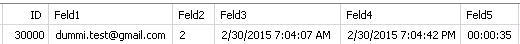
\includegraphics[width=\textwidth,height=\textheight,keepaspectratio]{graphics/trackingtableexample.png}
\caption{Example table entry}
\end{figure}
\newpage
The NavArCarData table stores all necessary information about the available cars which can be tracked.
\begin{figure}[htbp]
\centering
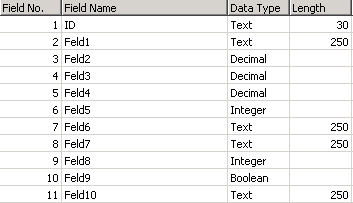
\includegraphics[width=80mm,height=\textheight,keepaspectratio]{graphics/cardatatable.png}
\caption{NavArCarData table}
\end{figure}
\\
The following figure of a entry consists of a unique car ID, car name, car price, leasing car price, monthly leasing price, horse power(hp), engine , motor fuel, number of doors, parking sensors and color. 
\newline  
\begin{figure}[htbp]
\centering
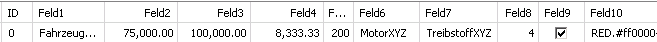
\includegraphics[width=\textwidth,height=\textheight,keepaspectratio]{graphics/cardatatablentry.png}
\caption{Example table entry}
\end{figure}
\newpage
The NavArUserData table has four columns which are used for saving the google email address,a custom email address, a name and a surname.
\\
\begin{figure}[htbp]
\centering
\includegraphics[width=100mm,height=\textheight,keepaspectratio]{graphics/userdatatable.png}
\caption{NavArUserData table }
\end{figure}
\\
\begin{figure}[htbp]
\centering
\includegraphics[width=\textwidth,height=\textheight,keepaspectratio]{graphics/userdatatableentry.png}
\caption{Example table entry}
\end{figure}
\\
To provide access to these three tables a page for each table was created with the same structure as the tables.  
\newpage
\subsection{Web service}
The communication between the C\# application and the Navision server was achieved by a web service. The web service functionality is built in the Navision server and can be used to publish pages.A page was published for each of the mentioned tables of the previous chapter. 
\\\\
\begin{figure}[htbp]
\centering
\includegraphics[width=\textwidth,height=\textheight,keepaspectratio]{graphics/webservice.png}
\caption{published pages}
\end{figure}
\\\\
These pages can be accessed via the web service from other programs. The web service also provides methods for creating, reading, deleting and updating data.
An example for reading from and writing to a web service can be found in the chapter Streaming C\# Application.   
\newpage
%
% Chapter8
\chapter{Future enhancements and possibilities} \label{chapter:Future enhancement and possibilities}

The developed application can provide several possibilites for the future.
\subsection{Support for iOS and Windows phones/tablets }
The idea of the design of the application was to program platform independent as possible. The only platform dependent code is the code to access the Metaio SDK via Java. So it is possible to simply swap out the Java code with c code for the iOs operation system. It would be the same on Windows phones, however Metaio currently stopped developing the Metaio SDK for windows phones.
\subsection{Other market segments}    
The application was developed for the main purpose to display information from tracked cars.However the same code structure can be implied for several other market segments.For instance you could make a application which tracks food from a supermarket shelf and displays information about the product. Such as the name,nutrient content, price and custom offers.Another scenario could be shopping malls. In this approach the application could track clothes or toys and display information about them. These are just two examples to show the possibilities but there a lot more of them.    
\newpage%
% Chapter9
\chapter{Resume}\label{chapter:Resume}
The project NAVAR was a great success. Not only the implementation of the project but also the improvement of our knowledge and our skills to work as a team.
\\\\
Since the start of the project we were driven to do the best we can to make a outstanding project for ourselves, our client 4relation Consulting GmbH. and our school Technische Gewerbe Museum(TGM).We improved our skills in five programming languages, which are HTML, CSS, Java , Javascript and C\#. The team acquired know how in new technologies like Windows Azure, Microsoft Dynamics Navsion and augmented reality.   
We learned to coordinate with our project team and the client. Every team member had his own responsibilities, task and deadline when something should be done or implemented. This increased our self-reliance and time management.
\\\\
Our project had also setbacks but we never lost track and continued to work eagerly. With our mental focus and the goal to succeed we were able to hit every milestone on target without delays.With the cooperation with our client we were introduced to an unknown world, the business world. 
\\\\
This unique experiences and challenges could never be achieved by typical school lessons. So we are proud and thankful that we had the opportunity to do such an amazing project. As we now look back at the start of the project we are amazed what a small group of students can create in such a short period of time.                 
\clearpage%

\include{tex/Fegerl Michael}


\addcontentsline{toc}{chapter}{Glossary} 
\printglossary[type=\acronymtype]
\glsaddall

\printglossary[type=\acronymtype]
%\printglossary[type=\acronymtype,style=listwithwidth]

%% include appendix
% Use of the sorted IEEE style, with changes:
% "dashification" was disabled


\cleardoublepage

% IEEE Style
\bibliographystyle{sty/IEEEtranS}

% GATHER
%\input "bib_file.bib"
\phantomsection{}
%\addcontentsline{toc}{chapter}{\bibname}
\pagestyle{myheadings}\markboth{\bibname}{\bibname}
\bibliography{tex/bib_file}

%%% generate index
%\clearpage%
%\markboth{\indexname}{\indexname}%
%\printindex%
%\addcontentsline{toc}{chapter}{\numberline{} %\indexname}%
%\addcontentsline{toc}{chapter}{\numberline{}\indexname}%

%% include affidavit
%



\end{document}
%%%%%%%%%%%%%%%%%%%%%%%%%%%%%%%%%%%%%%%%%%%%%%%%%%%%%%%%%%%%%%%%%%%%%%%%%%%%%%%%%%%%%%%%%%%%%%%%%%%
%%%%%%%%%%%%%%%%%%%%%%%%%%%%%%%%%%%%%%%%%% End Dokument %%%%%%%%%%%%%%%%%%%%%%%%%%%%%%%%%%%%%%%%%%%
%%%%%%%%%%%%%%%%%%%%%%%%%%%%%%%%%%%%%%%%%%%%%%%%%%%%%%%%%%%%%%%%%%%%%%%%%%%%%%%%%%%%%%%%%%%%%%%%%%%
